% The command below calls the preprint style^M
% which will produce a one-column, single-spaced document.^M
% Examples of commands for other sub-styles follow. Use^M
% whichever is most appropriate for your purposes.^M

%\documentclass[12pt,preprint]{aastex}
%\documentclass[iop,appendixfloats]{emulateapj}

% manuscript produces a one-column, double-spaced document:

%\documentclass[manuscript]{aastex}
%----------------------------------
% mn2esample.tex
%
% v2.1 released 22nd May 2002 (G. Hutton)
%
% The mnsample.tex file has been amended to highlight
% the proper use of LaTeX2e code with the class file
% and using natbib cross-referencing. These changes
% do not reflect the original paper by A. V. Raveendran.
%
% Previous versions of this sample document were
% compatible with the LaTeX 2.09 style file mn.sty
% v1.2 released 5th September 1994 (M. Reed)
% v1.1 released 18th July 1994
% v1.0 released 28th January 1994

\documentclass[useAMS,usenatbib]{mn2e}

% If your system does not have the AMS fonts version 2.0 installed, then
% remove the useAMS option.
%
% useAMS allows you to obtain upright Greek characters.
% e.g. \umu, \upi etc.  See the section on "Upright Greek characters" in
% this guide for further information.
%
% If you are using AMS 2.0 fonts, bold math letters/symbols are available
% at a larger range of sizes for NFSS release 1 and 2 (using \boldmath or
% preferably \bmath).
%
% The usenatbib command allows the use of Patrick Daly's natbib.sty for
% cross-referencing.
%
% If you wish to typeset the paper in Times font (if you do not have the
% PostScript Type 1 Computer Modern fonts you will need to do this to get
% smoother fonts in a PDF file) then uncomment the next line
% \usepackage{Times}

%%%%% AUTHORS - PLACE YOUR OWN MACROS HERE %%%%%
\usepackage{color}
\usepackage{graphicx}
\usepackage{amsmath}
\usepackage{amssymb}
\definecolor{orange}{rgb}{1,0.5,0}
%\usepackage[colorlinks=True,citecolor=orange,urlcolor=blue,linkcolor=red]{hyperref}

\newcommand{\figurepath}{.}


%  Definition of fonts


\newcommand{\tom}{\tilde{\omega}}

\newcommand{\ri}{r_{\rm i}}

\newcommand{\ro}{r_{\rm out}}

\newcommand{\rs}{r_{\star}}

\newcommand{\mj}{\dot{M}_{\rm jet}}

\newcommand{\ms}{\dot{M}_{\star}}

\newcommand{\vk}{v_{\rm K}}

\newcommand{\ti}{t_{\rm i}}

\newcommand{\rj}{R$_{\rm jet}$}

\newcommand{\rk}{R_{\kappa}}

\newcommand{\cs}{c_{\rm s}}

\newcommand{\css}{c_{\rm s}^2}

\newcommand{\bp}{B_{\rm P}}

\newcommand{\bh}{B_{\phi}}

\newcommand{\jp}{\vec{B}_{\rm P}}

\newcommand{\cm}{{\rm cm}}

\newcommand{\msun}{{\rm M}_{\sun}}

\newcommand{\rsun}{{\rm R}_{\sun}}

\newcommand{\rstar}{{\rm R}_{\star}}

\newcommand{\lumsun}{{\rm L}_{\sun}}

\newcommand{\lumstar}{{\rm L}_{\star}}

\newcommand{\lumdisk}{{\rm L}_{\rm disk}}

\newcommand{\etat}{{\eta}_{\rm t}}

\newcommand{\betat}{{\beta}_{\rm t}}

\newcommand{\betai}{{\beta}_{\rm i}}

\newcommand{\deltai}{{\delta}_{\rm i}}

\newcommand{\rhoi}{{\rho}_{\rm i}}
\newcommand{\refer}{{\color{orange}REFERENCE}}

% Bibliography and bibfile
\def\aj{AJ}%
          % Astronomical Journal
\def\actaa{Acta Astron.}%
          % Acta Astronomica
\def\araa{ARA\&A}%
          % Annual Review of Astron and Astrophys
\def\apj{ApJ}%
          % Astrophysical Journal
\def\apjl{ApJ}%
          % Astrophysical Journal, Letters
\def\apjs{ApJS}%
          % Astrophysical Journal, Supplement
\def\ao{Appl.~Opt.}%
          % Applied Optics
\def\apss{Ap\&SS}%
          % Astrophysics and Space Science
\def\aap{A\&A}%
          % Astronomy and Astrophysics
\def\aapr{A\&A~Rev.}%
          % Astronomy and Astrophysics Reviews
\def\aaps{A\&AS}%
          % Astronomy and Astrophysics, Supplement
\def\azh{AZh}%
          % Astronomicheskii Zhurnal
\def\baas{BAAS}%
          % Bulletin of the AAS
\def\bac{Bull. astr. Inst. Czechosl.}%
          % Bulletin of the Astronomical Institutes of Czechoslovakia 
\def\caa{Chinese Astron. Astrophys.}%
          % Chinese Astronomy and Astrophysics
\def\cjaa{Chinese J. Astron. Astrophys.}%
          % Chinese Journal of Astronomy and Astrophysics
\def\icarus{Icarus}%
          % Icarus
\def\jcap{J. Cosmology Astropart. Phys.}%
          % Journal of Cosmology and Astroparticle Physics
\def\jrasc{JRASC}%
          % Journal of the RAS of Canada
\def\mnras{MNRAS}%
          % Monthly Notices of the RAS
\def\memras{MmRAS}%
          % Memoirs of the RAS
\def\na{New A}%
          % New Astronomy
\def\nar{New A Rev.}%
          % New Astronomy Review
\def\pasa{PASA}%
          % Publications of the Astron. Soc. of Australia
\def\pra{Phys.~Rev.~A}%
          % Physical Review A: General Physics
\def\prb{Phys.~Rev.~B}%
          % Physical Review B: Solid State
\def\prc{Phys.~Rev.~C}%
          % Physical Review C
\def\prd{Phys.~Rev.~D}%
          % Physical Review D
\def\pre{Phys.~Rev.~E}%
          % Physical Review E
\def\prl{Phys.~Rev.~Lett.}%
          % Physical Review Letters
\def\pasp{PASP}%
          % Publications of the ASP
\def\pasj{PASJ}%
          % Publications of the ASJ
\def\qjras{QJRAS}%
          % Quarterly Journal of the RAS
\def\rmxaa{Rev. Mexicana Astron. Astrofis.}%
          % Revista Mexicana de Astronomia y Astrofisica
\def\skytel{S\&T}%
          % Sky and Telescope
\def\solphys{Sol.~Phys.}%
          % Solar Physics
\def\sovast{Soviet~Ast.}%
          % Soviet Astronomy
\def\ssr{Space~Sci.~Rev.}%
          % Space Science Reviews
\def\zap{ZAp}%
          % Zeitschrift fuer Astrophysik
\def\nat{Nature}%
          % Nature
\def\iaucirc{IAU~Circ.}%
          % IAU Cirulars
\def\aplett{Astrophys.~Lett.}%
          % Astrophysics Letters
\def\apspr{Astrophys.~Space~Phys.~Res.}%
          % Astrophysics Space Physics Research
\def\bain{Bull.~Astron.~Inst.~Netherlands}%
          % Bulletin Astronomical Institute of the Netherlands
\def\fcp{Fund.~Cosmic~Phys.}%
          % Fundamental Cosmic Physics
\def\gca{Geochim.~Cosmochim.~Acta}%
          % Geochimica Cosmochimica Acta
\def\grl{Geophys.~Res.~Lett.}%
          % Geophysics Research Letters
\def\jcp{J.~Chem.~Phys.}%
          % Journal of Chemical Physics
\def\jgr{J.~Geophys.~Res.}%
          % Journal of Geophysics Research
\def\jqsrt{J.~Quant.~Spec.~Radiat.~Transf.}%
          % Journal of Quantitiative Spectroscopy and Radiative Trasfer
\def\memsai{Mem.~Soc.~Astron.~Italiana}%
          % Mem. Societa Astronomica Italiana
\def\nphysa{Nucl.~Phys.~A}%
          % Nuclear Physics A
\def\physrep{Phys.~Rep.}%
          % Physics Reports
\def\physscr{Phys.~Scr}%
          % Physica Scripta
\def\planss{Planet.~Space~Sci.}%
          % Planetary Space Science
\def\procspie{Proc.~SPIE}%
          % Proceedings of the SPIE
\let\astap=\aap
\let\apjlett=\apjl
\let\apjsupp=\apjs
\let\applopt=\ao

\newcommand{\figpath}{/Users/bhargavvaidya/MyProject/work/Leeds_Uni/SiOJets_New/PAPER/PFIGS/}
%%%%%%%%%%%%%%%%%%%%%%%%%%%%%%%%%%%%%%%%%%%%%%%%

\begin{document}
%\title{SiO Molecular Jets around young stars - A numerical perspective}
\title[EHV SiO component in Molecular Outflows]{Synthetic Observations of Extremely High Velocity (EHV) SiO component
  in young molecular outflows}
\author[B. Vaidya, Tom Douglas, Paola Caselli]{B. Vaidya$^{1}$\thanks{E-mail:
B.Vaidya@leeds.ac.uk (BV)}, Tom Douglas$^{1}$, Paola Caselli$^{1}$\\
$^{1}$School of Physics and Astronomy, University of Leeds, Leeds LS2
9JT\\
}

\date\today

%\date{Accepted yyyy m dd. Received yyyy m dd; in original yyyy m dd}
\pagerange{\pageref{firstpage}--\pageref{lastpage}} \pubyear{yyyy}


\maketitle

\label{firstpage}

\begin{abstract}
  % context heading (optional)
  {A bipolar, collimated outflow is one of the first signposts of star
formation. As it propagates through the molecular
cloud, it injects energy and momentum via shocks 
and fosters chemical evolution by forming, destroying and entraining
molecules along its path.}  
  % aims heading (mandatory)
   {High 
velocity molecular outflows are extensively studied for both low mass
and high mass stars. They are usually observed using standard outflow and shocks
tracers like CO and SiO. However, the exact nature of
the excitation of these molecules is not yet clear due to lack of models that
simultaneously study the dynamics along with complex molecular chemistry.}
  % methods heading (mandatory)
   { For such a study, we have performed Magneto-hydrodynamic (MHD) simulations
of knotty jet propagation into a molecular cloud using the PLUTO
code. Firstly, we evolve the jet dynamical quantities in conjunction
with different non-equilibrium cooling prescriptions of varying complexities. 
The most complex is that of molecular cooling along with
H$_2$ chemistry. This prescription allows us to track the formation
and destruction of HI, HII and H$_2$ along with the flow dynamics. 
The final state of the jet obtained for each cooling model is then
given as an input to a radiative line transfer code to
obtain SiO emission maps, spectra and position-velocity (PV) digrams.}
  % results heading (mandatory)
   {Our model can successfully explain the signatures of extremely high
     velocity (EHV) emission of SiO seen in early outflows. In particular,
     the line intensities, spectra and PV diagrams obtained from our
     model are very similar to those observed in case of outflows with
     EHV emission. In addition, the Atacama Large Millimeter Array
     (ALMA) predictions for such
     early molecular outflows shows bright emission coming from young
     internal knots and bow shock due to thermal
     instability. Our multi-line modeling of SiO supports
     the observational feature seen in Herbig-Haro (HH 211)
     that higher line transitions trace
     regions close to the axis of the jet. The dependence of emission on
     different cooling prescription and abundance profiles is clearly
     outlined from our parameter study.}
  % conclusions heading (optional), leave it empty if necessary 
\end{abstract}

   \begin{keywords}
    MHD -- methods:numerical -- ISM: jets and outflows
   \end{keywords}


%
%

%===============================================================

\section{Introduction}
Jets are one of the first manifestations of star
formation in dense molecular cores. They are ubiquitous in both
massive and low mass star forming regions. These supersonic flows,
perpendicular to the underlying accretion disk, play a vital role in
removing excess angular momentum and thereby aiding in the accretion onto the protostar. 
For low mass stars, they are believed to be launched by magneto-centrifugally forces and
further collimated by magnetic hoop stress
\citep[][]{Blandford:1982p892, Konigl:2000p607}. However, in case of
high mass stars, radiative forces also contribute to flow dynamics
during the later evolutionary stages (\citealt{Vaidya:2011p8992}). 
Typically, these jets are a few parsec in size long and can be divided into
three length-scale domains, viz. source and disk scales (1-10$^{2}\,$AU),
envelope scales ($10^{2} - 10^{5}$\,AU) and parent cloud scales
($10^{5} - 10^{6}$\,AU) (\refer : Frank et. al, 2013, PPVI). Of these, it is at the envelope scale where rich chemical evolution occurs as the jet interacts
with the molecular medium. In this region, the jet propagates into a
relatively static medium inducing shocks that are interesting from both a
physical and chemical point of view. In addition to jets, molecular
material from the surroundings is entrained and accelerated to high
velocities giving rise to molecular outflows.
%

Bipolar molecular outflows from low and high mass stars
have been studied in detail over the past 
decade \citep[see reviews by][]{Bachiller:1996p4692, Beuther:2002p1149, Arce:2007p798,
Tafalla:2011p14051}. Advances in millimeter interferometers 
allow observations of these outflows with spatial resolution of a
few arc seconds. A large number of studies observing young
outflows are done using standard outflow and shock tracers,
e.g. CO and SiO respectively. In addition to these molecular tracers,
shocks from these outflows are detected in molecular hydrogen using
infra-red telescopes. Also, energetic outflows like that of
Orion source I show evidence of SiO masers very close to the launching
region of a MHD disk wind \citep{Goddi:2009p8571, Vaidya:2013p12777}. 
Based on these observational studies, various
empirical properties for these outflows have been discovered. 
For example, the high resolution interferometric studies with
CO (1-0) and SiO (2-1) have revealed highly collimated jet-like
outflows (with opening angles less than a few degrees); they are
referred to as {\em{molecular jets}}. HH 211 is the best example of
such a molecular jet (\citealt{Gueth:1999p4683}).
Episodic knots believed to be caused by variable accretion events are a common property
of young molecular outflows usually observed with higher line
transitions of CO and SiO (e.g. in L1577:
\citealt{Gueth:1998p14058}, in HH300: \citealt{Arce:2001p14064}). These knots show their signatures
as {\em{wedges}} in the PV diagrams \cite{Arce:2001p14065}. Also, 
observed in these outflows are signatures of rotation and
precession (for e.g., in DG Tau: \citealt{Bacciotti:2002p2084}).
%

Despite this large amount of data available, the exact nature of
molecular emission in outflows is not clear. For a complete understanding it is imperative
to complement these observations with theoretical models. Many models
based on hydro-simulations and steady state shock calculations
were proposed to explain the observational signatures of molecular
outflows. Among them the two main models are that of wide-angled wind
driven \citep{Shu:1991p14071} and jet driven outflow
\citep{Canto:1991p14123}. 
The most popular among them is the jet driven model as wind
driven molecular outflows not only fail to match observed PV diagrams (\citealt{Cabrit:1992p14098})
but also tend to sweep large quantity of material at the extremities
of the lobes (\citealt{Masson:1992p14101}), while the jet driven models could successfully
derive the global outflow shapes and mass velocity relations of CO
outflows \citep{Raga:1993p9948,
  Masson:1993p9661,Downes:2003p9946,Downes:2007p9514}. 
There have also been some attempts to combine these two
models into one (\citealt{Shang:2006p14268}) to explain the global observational features. 
However, most of these dynamical models do not
account for shock chemistry. Instead, shock chemistry is studied
independently using steady state non-dissociative C-type and
dissociative J-type shocks models \citep{Neufeld:1989p11689, Schilke:1997p14140,Flower:2003p11236}. 
The MHD calculations by \cite{Glassgold:1991p13703} suggested that molecules
like SiO and CO could form within the jet. Similar conclusions of
molecules surviving in steady state disk winds have also been shown
(\citealt{Panoglou:2012p10039}). 
Very few simulations have modelled the outflow
dynamics including molecular chemistry and in absence of
magnetic fields \citep{Raga:1995p12965, Smith:2003p9985}. 
Recent models have also incorporated
infall from the envelope \citep{Rawlings:2013p14920} and radiation
transfer \citep{Offner:2011p14861} to explain molecular 
emission from Class 0 protostellar outflow sources. 



%
In the present work, our goal is to take a step further in the modeling of
jet driven molecular outflows. The present model aims to consistently derive observed emission properties of molecular outflows, specifically various SiO line
transitions, by combining axisymmetric MHD simulations of
radiative jet propagation with time-dependent simple chemistry and 3D radiative
transfer. In particular, we evolve the jet dynamical
quantities in conjunction with different non-equilibrium cooling
prescriptions of varying complexities. The most complex is that of
molecular cooling along with hydrogen chemistry. This prescription
allows us to track the formation and destruction of 
HI, HII and H$_{2}$ along with the flow dynamics. 
The final state of the jet obtained for each cooling model is then
given as input to a non-LTE line radiative transfer code
to obtain emission maps, spectra and PV digrams. These emission maps
are further processed using the Common Astronomy Software Applications
package (CASA) to obtain synthetic ALMA images of the resultant molecular outflows.
%

In the next three sections~\ref{sec:numsetup}, \ref{sec:chem} and
\ref{sec:radtrans}, we describe our numerical setup, cooling
prescriptions and radiative transfer code respectively. In
sections~\ref{sec:parasurvey} and \ref{sec:results}, we will present results from the parameter survey and the
discussions along with predicted ALMA maps will be presented in
sections~\ref{sec:ALMAview} and \ref{sec:discussion}, followed by
conclusions in section~\ref{sec:conclusion}.

\section{Numerical Setup}
\label{sec:numsetup}
\subsection{Numerical code and Equations}
For our study, we carry out numerical axisymmetric ideal MHD simulations using the PLUTO code \citep{Mignone:2007p644} which is based on a conservative scheme of Godunov type.
We have modified the original code to incorporate molecular cooling
from self-consistent evolution of hydrogen chemistry (see Sect.~\ref{sec:chem}).

  
In general, the MHD code considers the following set of equations.
The conservation of the mass and the momentum,
%
\begin{equation}\label{masscons}
\frac{\partial \rho}{\partial t} + (\vec{v} \cdot \nabla)\rho  +
\rho \nabla \cdot \vec{v} = 0
\end{equation}
%
\begin{equation}\label{momcons}
\rho(\frac{\partial \vec{v}}{\partial t} +
(\vec{v} \cdot \nabla) \vec{v}) =
- \nabla P + \frac{1}{4\pi} (\nabla \times \vec{B}) \times \vec{B}
\end{equation}
%
where $\rho$ is gas density, $\vec{v}$ the velocity vector, $P$ the gas pressure,
and $\vec{B}$ the magnetic field vector with the poloidal and toroidal
components - $\vec{B}_{\rm p}, {B}_{\phi}$. Note that the forces due
to gravity are neglected for this problem as the domain of interest is
far away from the central object.  
%

The cooling function $\Lambda$ which depends on temperature $T$, mass density $\rho$ and
chemical abundances {\bf{X}}, appears in the
energy equation as a source term,

\begin{equation}\label{encons1}
\frac{\partial}{\partial t}(\rho E)
+ \nabla \cdot\left[ \rho E \vec{v} + (P + \frac{B^2}{8\pi})\vec{v}\right]  
- \vec{B}(\vec{v}\cdot\vec{B}) = -\Lambda(\rho,T,{\bf{X}}),
\end{equation}
%
%\begin{equation}\label{encons1}
%\frac{\partial}{\partial t}(\rho {\rm E}) + \nabla.\left[ (\rho
%{\rm E})\textbf{v} + (\textbf{P} + \frac{B^2}{8
%\pi})\textbf{v}\right] - \textbf{B}(\textbf{v.B}) = \rho\left[
%-\nabla\Phi + (\textbf{F}^{\rm rad})\right].\textbf{v}
%\end{equation}
%
where the total energy density of the flow $E$ comprises contributions from 
the internal energy $\epsilon$, the mechanical energy and the magnetic energy,
%
\begin{equation}\label{encons2}
 E = \epsilon + \frac{v^2}{2} + \frac{B^2}{8 \pi \rho}.
\end{equation}
The gas pressure in the flow is related to the density assuming an equation 
of state with the adiabatic index $\gamma$,
%
\begin{equation}\label{EOS}
P = (\gamma - 1) \rho \epsilon.
\end{equation}
The value of $\gamma$ is related to the degree of freedom for a
mixture of gas and thus depends on the composition and temperature.
We have adopted a constant value of 5/3 for the adiabatic index and
have described its consequences in the appendix (see ~\ref{sec:treatgamma}).

The evolution of chemical abundances for each species is solved via,
%
\begin{equation}\label{chemevol}
\frac{\partial \rho{\bf{X}}_{i}}{\partial t} + \nabla \cdot (\rho
{\bf{X}}_{i} \vec{v})  = \rho {\bf{S}}_{i},
\end{equation}
where ${\bf{S}}_{i}$ represents the net creation or destruction of a
given species through chemical reactions (see Sect.~\ref{sec:chem}).

The evolution of the magnetic field is governed by the induction equation,
%
\begin{equation}\label{induction}
\frac{\partial \vec{B}}{\partial t} = \nabla \times \left(\vec{v}\times \vec{B}\right).
\end{equation}
%
In addition to the above set of equations, the code obeys the condition of divergence-free 
magnetic fields, $\nabla \cdot \vec{B} = 0$, which is numerically achieved by construction 
using the Powell's eight wave formulation \citep{Powell:1999p14822}.

\subsection{Physical Model}
We model the propagation of an axi-symmetric jet
in (r,z,$\phi$) cylindrical co-ordinates as it interacts with the
ambient medium at distances $\gtrsim$ 1000\,AU. 
At these distances from the central source, the downward pull of gravity plays a
negligible role on the dynamics of the jet. The ambient medium with which the jet interacts primarily
represents the molecular cloud core. We study the interaction within a
radial extent of 20\,\rj\,\, and a vertical extent of 100\,\rj\,\,(\rj\,\, being the radius of
the jet). Numerically, it is resolved by an uniform grid with a domain
of 200$\times$1000 cells in the radial and vertical directions. For simplicity, we choose this medium
to be unmagnetized and non-turbulent. The density in the ambient
medium varies with vertical height $z$ as, $\rho_{\rm amb}\sim (\rho_0/z^{2})$
which is consistent with observations \citep{Keto:2010p15549,
  Caselli:2011p13935}. The value of
$\rho_0$ depends upon the density contrast, $\eta$, between the jet and
the ambient medium. The number density in the jet is kept fixed such
that the density in the ambient medium lies within a range of $10^{4}-10^{5}
\rm cm^{-3}$. The pressure in the ambient molecular medium is
set so to maintain a constant temperature of 50\,K. Note, dense
molecular cores through which young outflows propagate
have lower temperatures ranging from 10-20\,K
(\citealt{Rathborne:2007p15753}). As the jet is hypersonic in both
cases, runs with lower ambient temperature of 10\,K do not show any 
appreciable changes in final dynamical structure of the jet.

%

The jet enters into the medium through a nozzle of radius \rj\,\,
from the lower boundary (z = 0). Optically visible jets from T-Tauri
stars are just about spatially resolved for the nearest
star forming regions i.e, their radii are of the order of
100\,AU at a few thousand AU from the source \citep{Ray:2012p15733}.
These jets have mass outflow rates of 10$^{-7}$ M$_{\odot}$
yr$^{-1}$ \citep{Dougados:2010p15774}. Younger and 
embedded jets in their Class 0 phase have
outflow rates about 10-100 times higher than 
corresponding jets from optically visible young stars
\citep{Bally:2007p2340, Dionatos:2009p15670, Ray:2012p15733}. Also,
these optically obscure jets are relatively slower with velocities
ranging around 100 km\,s$^{-1}$ \citep{Bally:2007p2340} as compared to
optically visible flows with velocities up to 500\,km\,s$^{-1}$
\citep[e.g,][]{Mundt:1987p15799}.
For the present model, the jet is injected into the domain with a 
velocity of $v_{\rm jet,0}$ = 100 km/s and the jet density is set to
$10^{5} \rm cm^{-3}$ within a jet radius of $2.5\times10^{15} \rm
cm$. With these choices we obtain a mass outflow rate of 10$^{-6}$
M$_{\odot}$ yr$^{-1}$, consistent with young jets. Most of the young outflows 
show variable features possibly due to variable accretion rates
or internal shocks inside the jet \citep[e.g.][]{Bachiller:1996p4692}.
We replicate such variability by superimposing the constant jet
velocity with sinusoidal pulsation with an amplitude of 25
km\,s$^{-1}$ with a periodicity of 70\,yr such that the dense knots
are separated by a distance of $\sim$\,1000\,AU.

Thermal and magnetic properties of jets from young stars are difficult
to constraint because of their large variation not only within the jet
but also in its surroundings. Forbidden line emissions from
HH objects indicate excitation temperatures of the order
of $\leq$10$^{4}$\,K \citep{Podio:2006p15921,
  Bally:2007p2340}. However, in case of 
young jets the temperature is
considerably lower (i.e, by an order of magnitude) than found in jets from Class I/II
sources as derived from various atomic lines in molecular jets from
L-1448C and HH211 \citep{Dionatos:2009p15670,Dionatos:2010p15968}.  
The temperature at the jet
nozzle for our model has been set to 1000\,K. Thus, the jet is
over-pressured by 60 times as compared with the ambient medium,
assuming $\eta$ = 3.0. Inside the jet beam, a radial variation of thermal
and magnetic pressure is adopted to maintain a magneto-static
equilibrium for all our runs (\citealt{Stone:2000p2650}). 
Based on these profiles, 
the toroidal magnetic field is assumed to be
zero at the axis and achieves a maximum at radius, $r_{\rm m} \sim 0.8$\rj\,\,
inside the jet. Though measuring magnetic fields in
most jets is not possible via unpolarized nebular lines, in some special
cases like HH 34S and HH 111V, it has been measured to be 10 and 30
$\mu\,G$ respectively \citep{Morse:1993p15960}. Considering the
dependence of such weak magnetic fields on density and radial distance in velocity-variable flows, 
\cite{Hartigan:2007p15768} has shown that at large distances from the 
star these fields only play a minor role in the dynamics. Thus for all
our runs the value of magnetic field strength, $B_{\phi}(r_{\rm m})$ 
is set to be $\sim 37\mu\,G$.
%

In order to consistently model the SiO emission arising from shocks as
this jet interacts with the medium, we evolve the dynamics along with
chemistry and cooling prescriptions. They are described in details in
the next section.

\section{Chemistry and Cooling}
\label{sec:chem}
\subsection{Molecular Chemistry}
\label{ssec:molcool}
Typically, early collimated outflows have cooling times shorter than
the dynamical times, implying that the radiative cooling plays a vital
role in their dynamics. In order to study such outflows it is necessary to evolve
the dynamics in conjunction with full molecular chemistry and
associated radiative processes. However, evolving a full complex
network of chemical equations along with dynamics is a very
computationally intensive task. As a result, we have focused only in
evolving the chemical equations pertaining to atomic and molecular
hydrogen. This prescription of molecular cooling has been added to the PLUTO
code to study the chemical evolution of molecular outflows during the
very early phases of star formation. In particular, the total hydrogen
number density n$_{\rm H}$ comprises of contribution from atomic and
molecular hydrogen i.e., n$_{\rm H}$ = n$_{HI}$ + n$_{H2}$. Whereas
the contribution to electrons comes from the ionized hydrogen, n$_{\rm HII}$ and
from negligible but fixed fraction of metals ($Z \sim 10^{-4}$).
%
Numerically, the
non-homogenous parts of the equations~\ref{encons1} and \ref{chemevol} 
are solved separately from the advection step
using operator splitting. Further, the rate equations are evolved at each advection time
step using sub-stepping and adaptive Runge-Kutta methods.
The formation and destruction of
fractions (denoted by \textbf{X}$_{i}$ in eq.~\ref{chemevol}) of three species, viz., fHI, f$H_{2}$
and fHII are tracked by the code based on the temperature dependent reaction rates
whose coefficients are specified 
in the Table~\ref{tab:chemeq} along with their literature references. 

%and shown in the left panel
%of figure~\ref{fig:tempvar}. The figure clearly shows that below
%1000\,K, the rate coefficient of radiative recombination is the
%most dominant. However at these temperatures, very few
%electrons and ionized hydrogen are present in the initial ambient
%medium, thus the corresponding rate for this reaction is not that
%significant initially. At low temperatures corresponding to the molecular
%cores, the rate of formation of molecular hydrogen dominates over other
%chemical processes, whereas for gas temperatures $>$ 1000\,K there exists a competition
%of different chemical processes elucidating the complex chemical interplay.

\begin{figure}
% 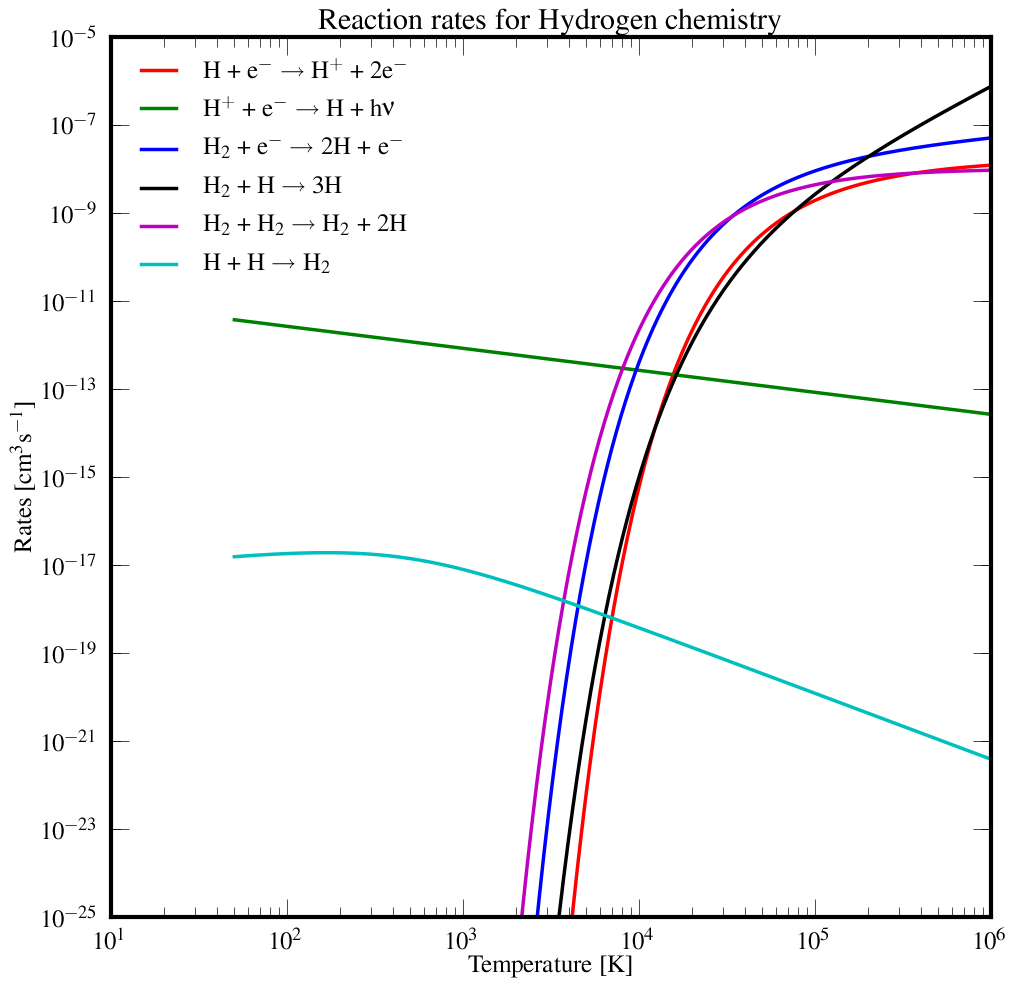
\includegraphics[width=1\columnwidth]{\figpath/H2ReactionRates_paper.png}
 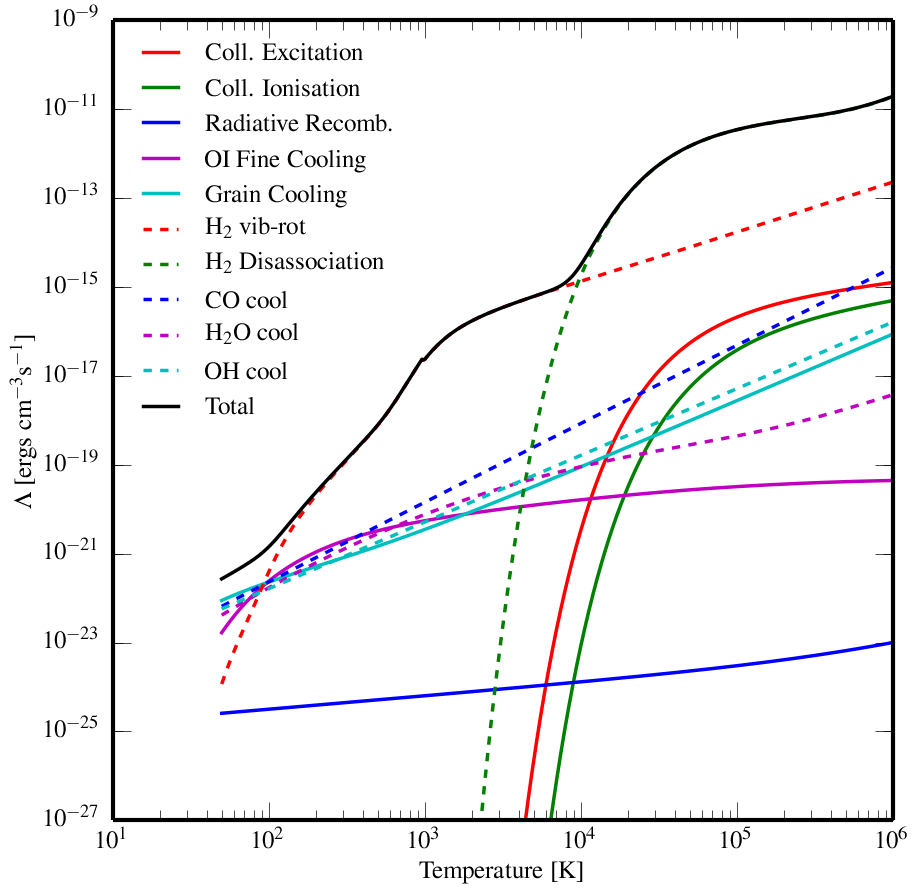
\includegraphics[width=1\columnwidth]{\figpath/H2CoolingFuncs_full.png}
 \caption{Variation of the cooling
   function $\Lambda(n,T,{\bf{X}})$ with temperature for the initial
   state.}
\label{fig:tempvar}
\end{figure}

\begin{table*}
\begin{minipage}{\textwidth}
\caption{Summary of the chemistry reaction set. T is the temperature
  in Kelvin, $T_{\rm eV}$ is the temperature in electron-volts, $T_{5}$
  = $T/1\times10^{5}$  and 
$T_{2}$  = T/100}
\label{tab:chemeq}
\begin{tabular}{l l l l}
\hline
No. & Reaction & Rate Coefficient ($\rm {cm}^{3} s^{-1}$) &
Reference~\footnote{REFERENCES -- (1) \cite{Cen:1992p13616} [Eq. 26a];
  (2) \cite{Woodall:2007p13623} [UMIST Database] (3)
  \cite{Galli:1998p13066} [Eq. H17]; (4) \cite{Abel:1997p12836}
  [Tab. 3 Eq. 13]; (5) \cite{Hollenbach:1979p12707} [Eq. 3.8]}\\
\hline
1. & H + e$^{-}$ $\rightarrow$ H$^{+}$ + 2e$^{-}$ & $k_1$ = $5.85
\times 10^{-11}$ $T^{0.5}$ \rm{exp}(-157,809.1/T)/(1.0 + $T_{5}^{0.5}$) & 1\\
2. & H$^{+}$ + e$^{-}$ $\rightarrow$ H + h$\nu$ & $k_2$ =
$3.5\times10^{-12} (T/300.0)^{-0.8}$ & 2\\
3. & H$_{2}$ + e$^{-}$ $\rightarrow$ 2H + e$^{-}$ & $k_3$ =
$4.4\times10^{-10} T^{0.35} \rm{exp}(-102,000.0/T)$ & 3\\
4. & H$_{2}$ + H $\rightarrow$ 3H & $k_4$ = $1.067\times10^{-10}
T_{\rm eV}^{2.012}(\rm{exp}(4.463/T_{\rm eV})^{-1}((1. + 0.2472 T_{\rm eV})^{3.512})^{-1} $& 4\\
5. &H$_{2}$ + H$_{2}$ $\rightarrow$ H$_{2}$ + 2H & $k_5$ = $1.0\times 10^{-8} \rm{exp}(-84,100/T)$ & 2\\
6. & H + H $\overset{\rm dust}\longrightarrow$ H$_{2}$ & $k_6 =
3.0\times10^{-17}\sqrt{T_{2}}(1.0 + 0.4\sqrt{T_{2} + 0.15} + 0.2T_{2} + 0.8T_{2}^{2})$ & 5 \\
\hline
\end{tabular}
\end{minipage}
\end{table*}

\subsection{Cooling Prescriptions}
%
Figure~\ref{fig:tempvar} shows the variation
of the cooling function, $\Lambda(\rho,T,{\bf{X}})$, with gas
temperature assuming conditions of initial ambient density. 
Various processes that contribute to the cooling function in our model
are listed in the figure. The formulations of these contributions
are adopted from \citep[][and references therein]{Smith:2003p9985, OSullivan:2009p10078}.
For low temperatures, we also 
take into account contribution to cooling function from molecules like
CO, whose abundance with respect to $n_{\rm H}$ is fixed to a
value of 10$^{-5}$ as measured in dense cores like L1544 \citep{Keto:2010p15549}. 
For each of the other molecules contributing to the cooling function (like OH, H$_{2}$O and atomic OI)
the abundance is fixed to values of $5\times10^{-6}$. Note, the
uncertain abundance values are rather arbitrary for these molecules. 
However, their contribution is only important when temperature is $<$
100\,K as seen in figure~\ref{fig:tempvar}. As the internal shocks, where most
of the molecular hydrogen is produced maintain temperatures higher
than 100\,K and densities $\sim$10$^{6}$ cm$^{-3}$, cooling due to these molecules do not
play a significant role even if the arbitrary abundance is increased
by a factor of 10 \citep{Smith:2003p9985}. Instead, a substantial contribution to the cooling
function, between T = 100\,K and 3000\,K, 
comes from the vibrational and rotational transitions of
molecular hydrogen plays and a very crucial role during the jet
evolution. Whereas, for temperatures above 3000\,K the
cooling is mainly via H$_{2}$ disassociation. The total curve for the
whole temperature range obtained in our runs is shown in black.
The fact that the initial ambient medium is largely molecular, cooling is also dominated by
molecular processes. In our reference model (see ~\ref{ssec:refrun}), 
we update this curve at each time step based on the fraction of
various hydrogen species. Thus during the evolution, even
contributions from collisional ionizations and excitations also become
important in regions dominated by atomic and ionized hydrogen.
%

We also ran simulations of axisymmetric MHD jets
with optically thin cooling prescriptions already existing in the public
release of the PLUTO-4 code. They are power-law cooling, 
simplified non-equilibrium (or atomic) cooling and tabulated
cooling. While these additional cooling prescriptions may not be a complete description of
the chemical and radiative processes in early outflows, they are ideal
to compare the results obtained from the more consistent newly added molecular
cooling. In addition, we compare these radiative runs with an adiabatic jet 
to cover a wide spectrum of jet thermodynamics. 
Such a comparison is presented in section~\ref{ssec:coolres}.


\section{Radiative Transfer}
\label{sec:radtrans}
%Radiative transfer modeling used for post processing.

\subsection{The radiative transfer code} \label{subsec:radiative_transfer_code}
The radiative transfer program used is LIME (LIne Modeling Engine;
\citealt{Brinch:2010p13078}), which  calculates line intensities based
on a weighted sample of randomly chosen points in a continuous 3D
model. The method of selecting these points is given in section
\ref{subsec:gridding}. At each of these points, the density of the
main collision partner (equivalent amount of H$_2$, given by n(H$_2$)+
n(HI), assuming that ionized Hydrogen does not collide with SiO), gas temperature, velocity, molecular abundances and unresolved turbulent velocity are specified. These points are then smoothed by Lloyd's algorithm \citep{Lloyd1982} in order to minimise the variation in distance between points whilst keeping the same underlying distribution. These points are then connected by Delaunay triangulation and it is between the points connected by this method that photon are allowed to propagate (fig.~\ref{grid}). The level populations of the selected molecules are calculated at each of these points from collisional and radiative (de)excitation and the local radiation field is calculated. This is repeated 20 times with the populations of each level converging towards a single value. This number of iterations is sufficient for the signal to noise ratio of the level populations (as defined in \citealt{Brinch:2010p13078}) to exceed 1000 for 99\% of the points, ensuring that the simulation has converged on a stable level population. After 20 iterations the model is ray-traced in order to produce synthetic brightness maps. The average of ten separate runs was taken to minimise the artefacts in the output images, resulting from the grid construction.% (Fig.~\ref{points}).


\begin{figure}
 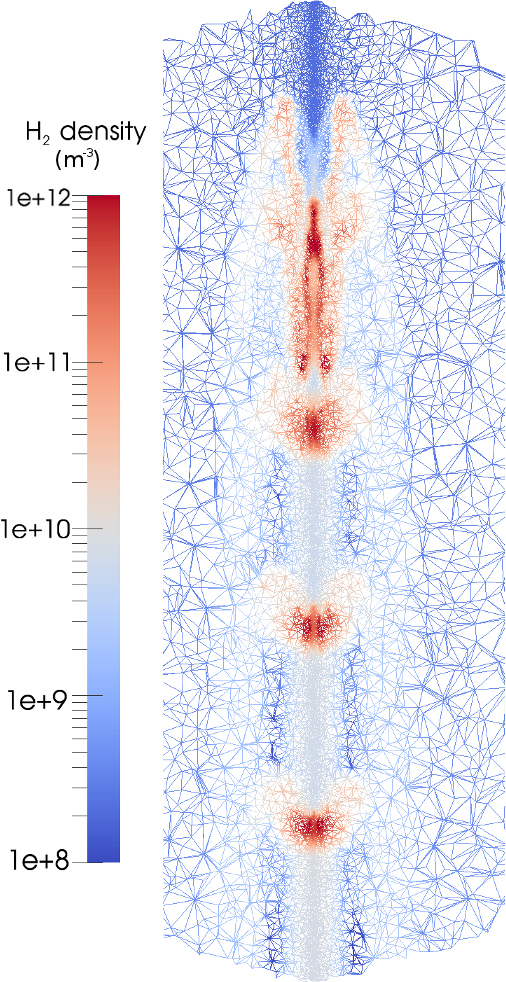
\includegraphics[width=84mm]{\figpath/grid.png}
 \caption{A plot of the points selected by the gridding process and the paths down which photons can propagate for points in the r,z plane. The points are color coded by the density distribution (in m$^{-3}$, as used in LIME) and are more concentrated in the high density knots.}
\label{grid} % This plots has to be changed. 
\end{figure}

\subsection{Grid construction} \label{subsec:gridding}
In order to construct the grid, candidate points are randomly selected from the volume to be simulated. These candidates then have their equivalent H$_2$ number density, and the number density of SiO, compared against those of a reference point in order to decide if the candidate point is to be used in the grid or not. Candidate grid points are selected at random in a cylindrical coordinate system that is linearly spaced in z and $\theta$ and logarithmically spaced in r. For each point to be selected, a random number $\alpha$ is drawn from the semi-open set [0,$\,$1) as a threshold. After selection of random coordinates, the H$_2$ density and SiO density at the candidate point (n and m, respectively) are compared against the densities of a reference point in the un-perturbed ambient medium multiplied by a factor of $\frac{4\eta}{5}$ (n$_{ref}$ and m$_{ref}$), where $\eta$ is the density contrast between the jet and ambient medium. If $\alpha<\left( \frac{n}{n_0} \right)^{0.3}$ or $\alpha< \left( \frac{m}{m_0} \right)^{0.3}$ then the point is selected for use. Otherwise another r, $\theta$, z co-ordinate is selected and it becomes the candidate point. In addition to this method of selection, 5\% of the points are linearly distributed in x, y and z with no bias with regards to density or abundance. This provides a minimum level of sampling for the large low density regions in the outer parts of the simulated volume. %See fig. \ref{points} for an example of the points distribution in r, z. The function comparing the candidate point to the reference point and the candidate point distribution were selected empirically to sample all scales while ensuring that the majority of points are located in the inner disc where the density is higher.
\smallskip

\subsection{SiO abundance}
\label{ssec:sioabun}
Molecular abundance is one of the important ingredients that is
required by the radiative transfer code described above. 
Typically, extremely low abundance of SiO is
found (n(SiO)/n(H2) $< 3\times10^{-12}$) in dark, dense clouds such
as TMC1 \citep{Ziurys:1989p14699,MartinPintado:1992p14309}. Whereas, in
outflows like L1448, SiO abundance can increase up to 10$^{-6}$ especially in
molecular bullets moving with a projected velocity of 60
km\,s$^{-1}$ \citep{Dutrey:1997p11185}. Thus, there is
an increase of 6 orders of magnitude from quiescent clouds
to outflows. Production of
gaseous SiO due to slow C-type shocks has been suggested to occur via release of
silicon from grain cores and from grain mantles. Various stationary
shock models indicate a sudden abundance increase in SiO 
near a shock speed of 20-30\,km\, s$^{-1}$. However, several young
outflows have velocities of the order of 100 km\,s$^{-1}$ as in the present
case. Shocks due to such outflows will dissociate H$_{2}$ and will
become J ({\em{jump}}) type shocks. Thus, molecules observed in such
energetic outflows must have been reformed in the flow as suggested by
detailed models of J-shocks by \cite{Neufeld:1989p14322}. SiO formation in J shocks
has also been modelled recently and has thought to be the source of
the SiO line emission observed in molecular outflows and jets
\citep{Guillet:2009p11229}.
%

In-spite of all numerical models relating to the study of enhancement
of SiO in shocks, very little is known about the dependence of SiO
abundance on shock speeds. Considering the complex grain
chemistry that is involved in order to estimate the functional
dependence of SiO abundance on shock speeds, we prescribe these
profiles based on limited empirical evidences. The most simple among
them is the top hat profile in which the SiO abundance is a low value of
10$^{-12}$ below 20 km s$^{-1}$ and above 100 km s$^{-1}$ and a
maximum value of 10$^{-6}$ between these two velocities.
Shock velocities $>$ 100 km s$^{-1}$ can lead to the 
ionisation of hydrogen and thereby effectively reduce the number
of collision centers for SiO resulting in a weaker emission. 
However, we also consider a step function dependence of SiO abundance
on shock velocity to incorporate cases where we allow for reformation
of atomic and molecular species.
In order to get rid of a discontinuous change of abundance, we also
prescribe a gaussian such that the peak SiO abundance of 10$^{-6}$ is at
60\,km\,s$^{-1}$, while the value of n(SiO)/n(H$_{2}$) falls below
10$^{-9}$ at 20 and 100 km s$^{-1}$. Such a huge variation in SiO
abundance may indeed be the case in regions where SiO is seen
in widespread \citep[e.g.,][also see section~\ref{sec:discussion}]
{Lefloch:1998p13983}. Also along with a Gaussian profile, we consider
the case where we extent the abundance of 10$^{-6}$ beyond 60 km\,s$^{-1}$. 
These functional dependences of SiO
abundance on shock velocity are shown in figure~\ref{abun}.  
In addition to this, if the temperature at the point is greater than
92,000\,K (the temperature of the Si-O bond disassociation energy) 
the abundance is reduced to 0. 
%

 \begin{figure}
  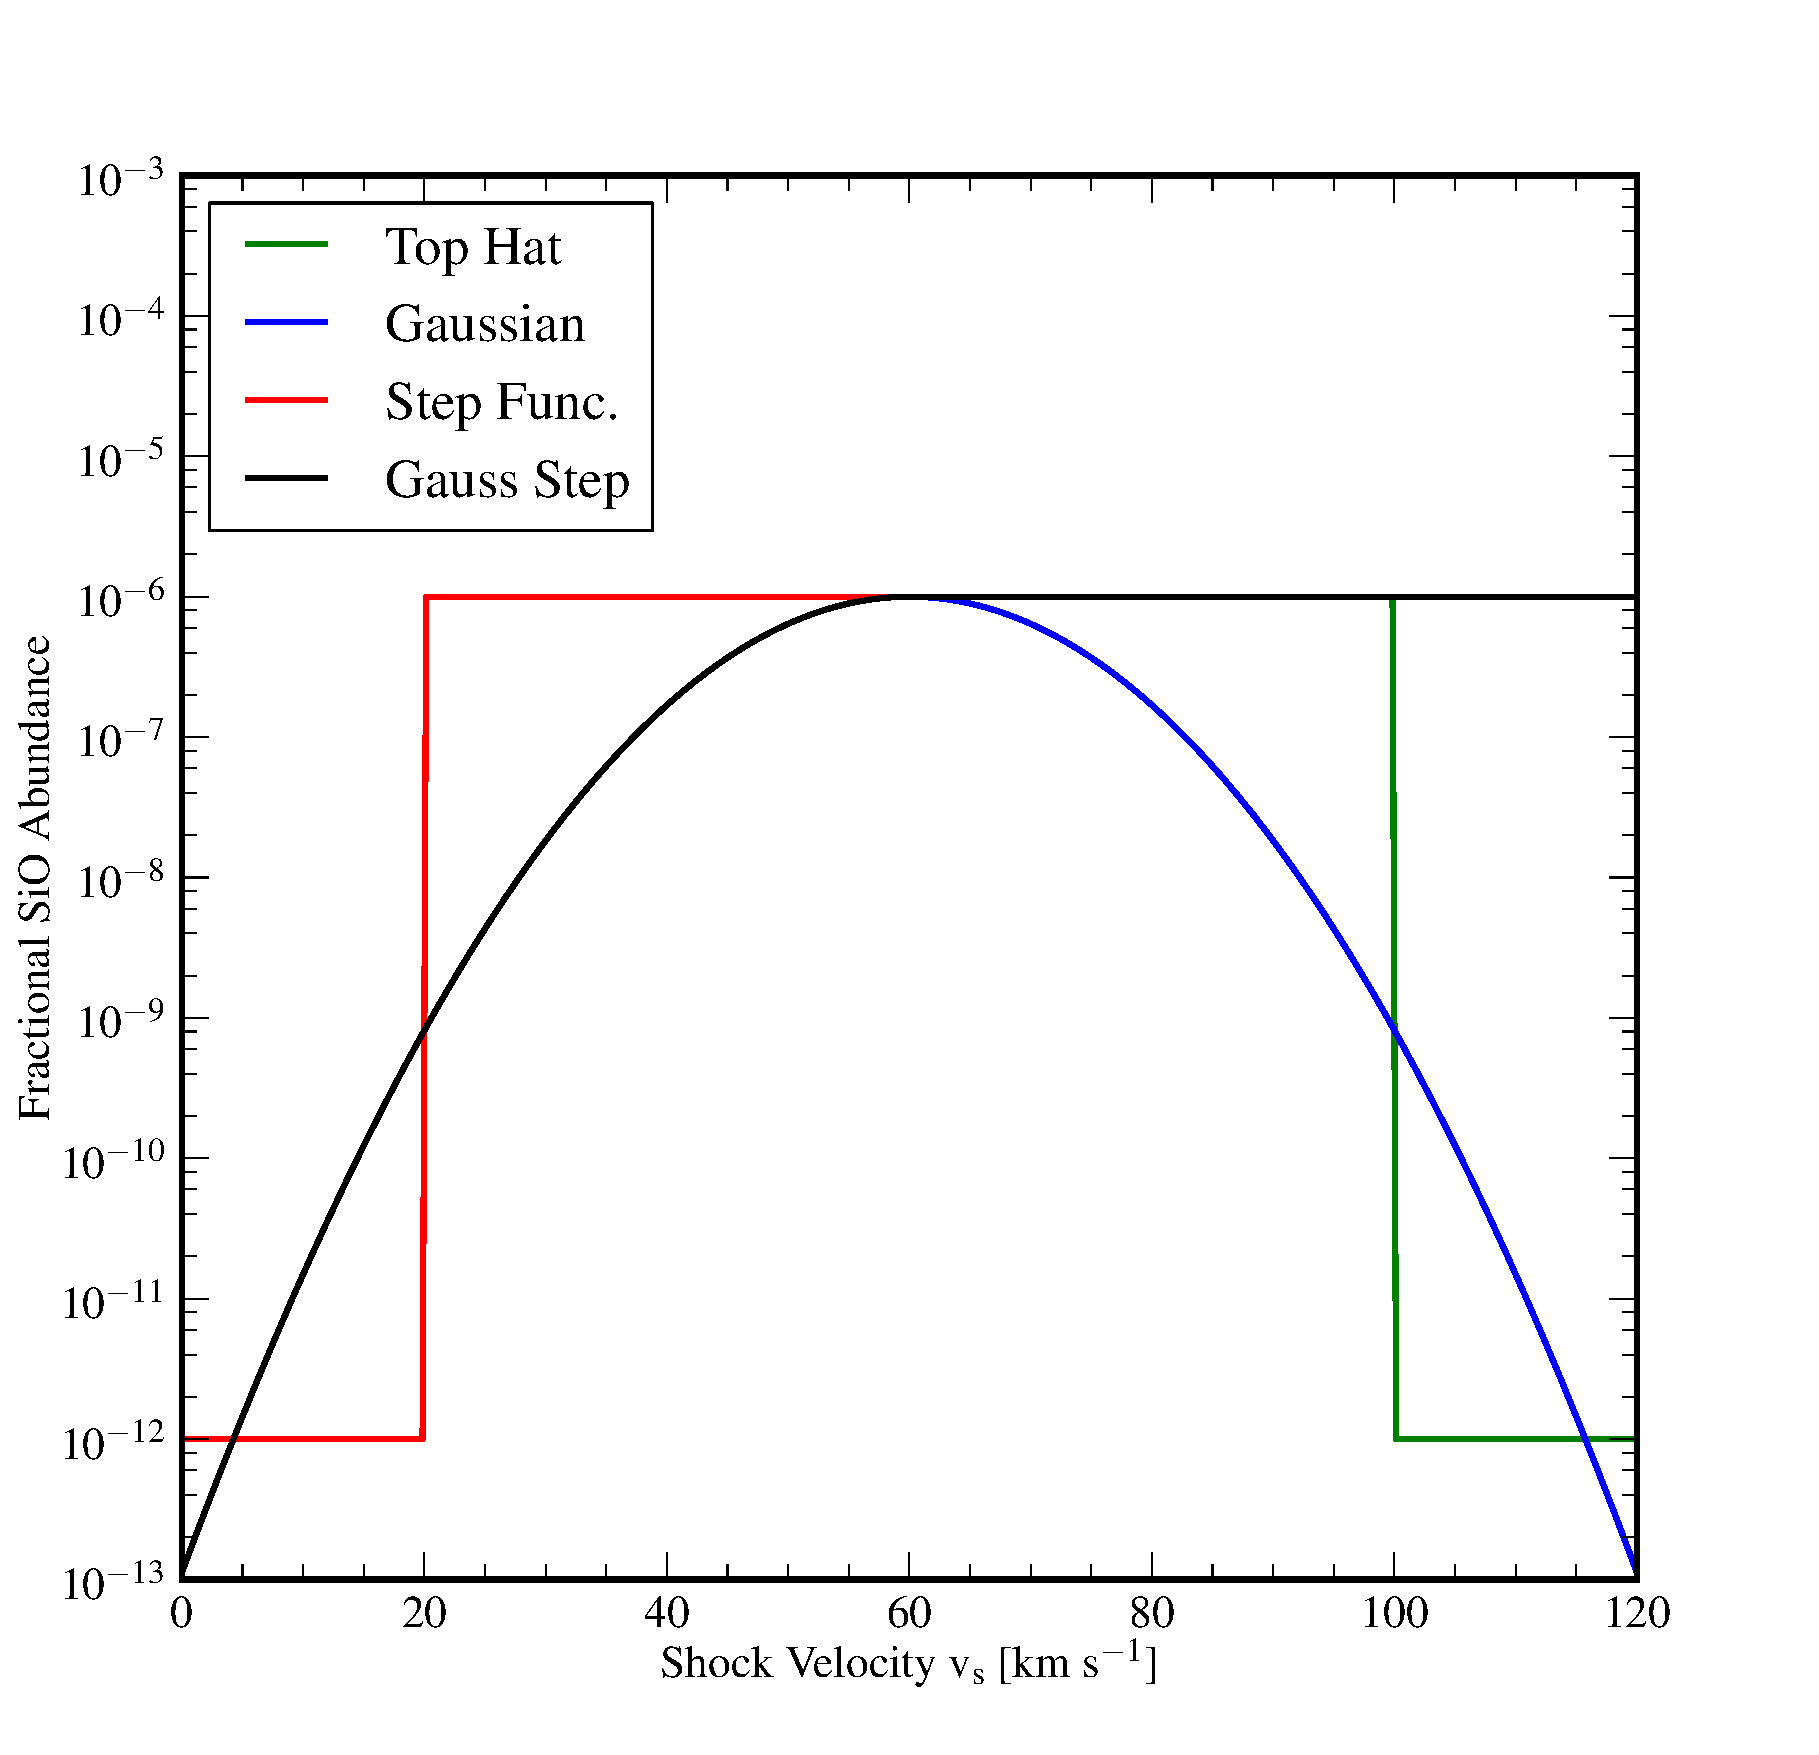
\includegraphics[width=1.\columnwidth]{\figpath/diffabun_profnew.pdf}%{\figpath/diffabunprof1.png}
  \caption{{\bf{CHANGEFIG}} The different fractional SiO abundances as a function of
    jet velocity, v$_{\rm jet}$.}
  \label{abun}
 \end{figure}

Further, the velocities obtained from the dynamical simulations are in fact the
jet flow velocities. They can well be different from the shock
velocities depending upon the density contrast between the jet and
ambient medium. For the present study, we will consider two
cases. Firstly, the most simple one in which the jet flow velocity is
same as the shock velocity. Considering that there is a density
contrast in the simulation setup, this assumption will
overestimate the shock velocity. We also
consider a case in which the shock speed of a dense plug accumulated
between the jet and medium is estimated by balancing the respective ram
pressures \citep{Masson:1993p9661},
\begin{equation}
\label{eq:shockjetvel}
v_{\rm s} = \frac{v_{\rm jet}}{1 + \eta^{-0.5}} = v_{\rm jet}\delta
\end{equation}
where v$_{\rm s}$ is the velocity of dense plug and v$_{\rm jet}$ is the
jet velocity. A comparative view of using such velocity corrections and
functional forms of SiO abundances are discussed in
Sec~\ref{ssec:sioabunem}.

    

% The fractional abundance is given by the equation:

% \begin{eqnarray}
% log(X)=-2.48\times10^{-8}v^5 + 5.50\times10^{-6}v^4 \nonumber \\
% - 4.28\times10^{-4}v^3 + 1.24\times10^{-2}v^2 \nonumber \\
% + 2.52\times10^{-2}v - 1.20\times10^{1}
% \label{eq:fracSio}
% \end{eqnarray}

% where v is the shock velocity in kilometres per second. 




\section{Parameter Survey}
\label{sec:parasurvey}
The results and analysis for the present work are divided in two parts,
viz., the dynamical numerical simulations and the
radiative transfer analysis. For each part we have used certain parameters
and the effect of changing them is studied. Ideally all these parameters should come from observational
results. However, not all quantities needed for our study are well
constrained by observations, thus they are considered as
free parameters. Such a parameter survey provides better handle on the range of allowed
values on qualitative comparison with observations. 
%

\subsection{Parameter definitions}
\label{ssec:paradef}
For the first part of the study concerning the dynamical numerical
simulations, we will focus on two main parameters. They are the
prescription of cooling and the density contrast between the jet and
the ambient medium denoted by $\eta$. The various cooling prescriptions used for the present study are
described in detail in section~\ref{sec:chem}. They differ in the
physical process that is responsible for cooling and chemistry. The
most simple one is that of power-law cooling with no chemistry and the
most complex cooling module is where molecular hydrogen chemistry is
evolved with contributions to cooling from other abundant molecules
like CO, OH etc. 
%

A value of $\eta > 1$, means that
that jet is over dense with respect to the medium. In all our runs with
different cooling prescriptions, we have assumed the jet to be
over-dense by 10 times compared to the ambient medium. Additionally, for
the atomic, tabulated and molecular cooling runs (see section~\ref{sec:chem}
for description of different cooling prescriptions) we have also used a
value of $\eta$ of the order of unity indicating similar densities in
the jet and the medium. Table~\ref{tab:result1} lists all the runs with
varying $\eta$ and cooling prescriptions, along with the peak
intensity and line widths at the bow shock.
%

To obtain the SiO emission maps and corresponding
spectra, two additional free parameters are required along with other
inputs described in section~\ref{sec:radtrans} . They are
the fractional abundance profile of SiO and the angle of inclination with
respect to line of sight denoted by $\phi$. Section~\ref{ssec:sioabun}
describes all the profiles used for the present study. $\phi$ = 90$^{\circ}$ indicates that
the outflow is in the plane of the sky. 
Additionally, we have used two other angles of inclination apart from the
plane of the sky, i.e, $\phi = 45^{\circ}, 60^{\circ}$ to compare
results with observations. The runs with different fractional
abundance profiles are described in table~\ref{tab:result2}. A
parameter introduced here is $\delta$ which is essentially the ratio
of shock velocity v$_{\rm s}$ and physical jet velocity v$_{\rm
  jet}$ such that its value depends on density contrast $\eta$
(see Eq.~\ref{eq:shockjetvel}).

\begin{table*}
\centering
\caption{Summary from parameter runs. The parameter $\delta$, is the ratio of
  shock to jet velocity and it depends on the density contrast $\eta$
  as shown in eq.~\ref{eq:shockjetvel}}
\begin{tabular}{c | c | c | c | c | c | c }
\hline
Run & Cooling Mode & $\eta$ & \multicolumn{2}{|c|}{Top Hat Profile
  $\delta = 1$} & \multicolumn{2}{|c|}{Gaussian Profile $\delta =
  1$}\\
\hline\hline
&&& $\int T_{\rm MB}dV$ [K-km\,s$^{-1}$] & $\Delta$v [km s$^{-1}$] & $\int T_{\rm MB}dV$ [K-km\,s$^{-1}$] & $\Delta$v [km s$^{-1}$] \\
\hline
adi10 & Nil (Adiabatic) & 10 & 2.91 & $>$40 & 0.25 & 40.0 \\
pow10 & Power law & 10 & 0.64 & 8.0 & 0.02 & 10.0\\
atm10 & Atomic & 10 & 2.04 & 36.0 & 0.58 & 38.0 \\
atm2 & Atomic & 2 & 3.21 & 18.0 & 0.64 & 20.0 \\
tab10 & Tabulated & 10 & 0.75 & 11.0 & 0.09 & 10.0 \\
tab2 & Tabulated & 2 & 2.89 & 8.0 & 1.0 & 9.0 \\
mol10 & Molecular & 10 & 1.10 & 10.0 & 0.1 & 11.0 \\
mol3 & Molecular & 3 & 3.3 & 14.0 & 0.66 & 12.0\\
\hline
\end{tabular}
\label{tab:result1}
\end{table*}


 

\begin{table*}
\centering
\caption{Summary of radiative transfer runs with different SiO fractional abundance
  profiles for dynamical simulation with molecular cooling and
  $\eta=3$. The integrated intensity assuming a single disk
  observation with a beam width of $15\,\arcsec$ is listed along with the
  corresponding spectral width.}
\begin{tabular}{l | l | l | l | l}
\hline
Profile & $\delta$ = v$_{\rm s}$/v$_{\rm jet}$ & $\int T_{\rm MB}dV$
[K-km\,s$^{-1}$] & $\Delta$v [km s$^{-1}$]\\ 
\hline\hline
Top Hat & 1.0 & 3.3 & 14.0 \\
Top Hat & 1/$(1.0 + \eta(z)^{-0.5})$ & 4.9 & 14.0 \\
Gaussian & 1.0 & 0.66
& 12.0 \\
Gaussian & 1/$(1.0 + \eta(z)^{-0.5})$ & 1.1
& 12.0 \\
%Functional & 100.0 & $(1.0 + \eta(z)^{-0.5})$ &
%& \\
%Functional & 100.0 & $(1.0 + \eta(z)^{-0.5})$ &
%& \\
\hline
\end{tabular}
\label{tab:result2}
\end{table*}

\subsection{Reference Run}
\label{ssec:refrun}
We define a reference run in order to quantify and compare results obtained from such a
survey of above mentioned parameters. The results shown in this work will be
pertaining to the reference run (unless otherwise mentioned) and appropriate comparison will be
discussed with other runs. 

The reference run in our calculation has density contrast $\eta$ = 3
with the initial jet density of 10$^{5}$ cm$^{-3}$. This jet enters the
ambient medium with a velocity of v$_{\rm jet,0}$ = 100 km
s$^{-1}$ which is further superimposed by sinusoidal perturbations to
replicate dense knots. The maximum value of toroidal magnetic field is
set to be 37$\mu\,G$ at the base of the jet.
\cite{Dionatos:2009p15670} have detected atomic lines
towards a molecular jet from L1448-C indicating a presence of embedded
atomic jet at low excitation. Additionally, they also detect pure
rotational transitions from H$_{2}$ indicating presence of molecules
along with the atomic jet. Line ratios from this source indicate that the
atomic gas is characterized by an an ionization fraction of 1\%,
which is considerably less as compared to ionization fraction of
10-20\% measured in optical jets \citep{Bacciotti:1995p15970}.
Initial jet composition is prescribed
be 89\% atomic, 10\% molecular and 1\% ionized, in qualitative
agreement of above observational results. 
%

The cooling in the reference jet is via molecular cooling prescription, whereby
the initial hydrogen fractions are evolved using appropriate rate equations and with cooling 
contributions for abundant molecules like CO, OH
etc. The final state (at time $\sim$ 1000 yr), i.e, density, temperature and velocity obtained from this 
run are given as inputs to the radiative transfer code to obtain the observational features
corresponding to SiO molecule. 
For the radiative transfer calculation, the source in the reference
run is stationary and the jet is in the plane of the sky ($\phi =
90^{\circ}$). A gaussian profile without any upper cutoff is used for the fractional abundance
of SiO. Further, the shock velocity which determines
the fractional abundance, v$_{\rm s}$, is less than the jet velocity in the
flow, such that their ratio $\delta$ is given by
equation~\ref{eq:shockjetvel}, where $\eta$ is the density contrast as a
function of height from the base of the jet.

\section{Results}
\label{sec:results}
\subsection{Comparison of cooling prescription}
\label{ssec:coolres}
We have done a comparison study of jet dynamics with various cooling
prescriptions, which are described in
Sect.~\ref{sec:chem}. Figure~\ref{fig:coolcmpdyn} shows the density of the MHD
jet at time $\sim$ 1000 years for these different cooling
prescriptions. For this study, we have chosen a density contrast at the base of
$\eta$ = 10 between the jet and ambient medium.
It is clear from the figure~\ref{fig:coolcmpdyn}, that the cooling plays a
significant role in determining the structure of the jet. The jets
with no or very little cooling are much wider compared to
jets having dominant cooling. For example, the adiabatic jet
has the widest bow shock at its apex and has the most prominent shell
of processed material, also known as the cocoon,
around it. While the jet with atomic cooling has a rather conical
jet head with significantly less cocoon surrounding it. The cocoon is
almost absent from the narrow jet with tabulated cooling. Instead, the jet
seems to form a very high density shell due to cooling of the
processed ambient gas. Further, the jet with tabulated cooling is narrower than the jet with molecular cooling. This clearly
shows the feedback of chemistry on the cooling function. The cooling
terms for both these jets are the same to begin with, however,
for the molecular jet the cooling terms evolve with jet dynamics as the fraction of
various hydrogen species change over time. Whilst the terms remain fixed to initial values, shown in the fig~\ref{fig:tempvar}, for the jet with tabulated
cooling. Additionally, the material at the bow shock for the jet
with tabulated and molecular cooling condenses forming dense knots. 
Such a condensation is caused due to thermal instability and is 
a typical feature of axi-symmetric radiative jets 
\citep[see, for e.g,][]{Blondin:1990p2130,Cerqueira:1999p15052}.
%

The dynamical states for each of this cooling prescriptions are then 
given as inputs to the radiative transfer code to obtain integrated J = 2-$>$1 SiO emission
maps shown in figure~\ref{fig:coolcmpsio}. The differences in dynamical
features are also reflected in the corresponding SiO emission
maps. These maps are obtained assuming an angle of inclination of
90$^\circ$ using the top hat abundance
profile with $\delta = 1$. They are then placed at a distance of
100$\,$pc and convolved with a beam with FWHM of 2.0\arcsec in order
to create the maps shown. 
The emission from the jet with atomic
cooling is coming from the conical jet head and younger knots closer
to base of the flow. Additionally, features in the shell at Z $\sim$
60, 75 also show evidence of faint emission. In case of the jet with
power-law cooling the emission mostly arises from the
internal knots. 
The emission coming from jets with
tabulated and molecular cooling resembles that observed in young molecular outflows.
Also in these outflows, strong emission arises from the
condensation formed at the bow shock due to thermal
instability. 
%

In summary, different cooling prescriptions strongly influence the
dynamics of MHD jet propagation in particular the thickness and
structure of the bow shock. These dynamical differences are
also reflected in SiO emission maps. The molecular cooling in our
model consistently takes into account the feedback of temperature and
density variation to evolve the chemical species unlike the tabulated cooling
where the fraction of chemical species remains fixed. Thus, for our reference
run we will adopt the molecular cooling prescription and compare
results with observations. The properties of
molecular cooling flows are described in details in the next section.

\begin{figure*}
 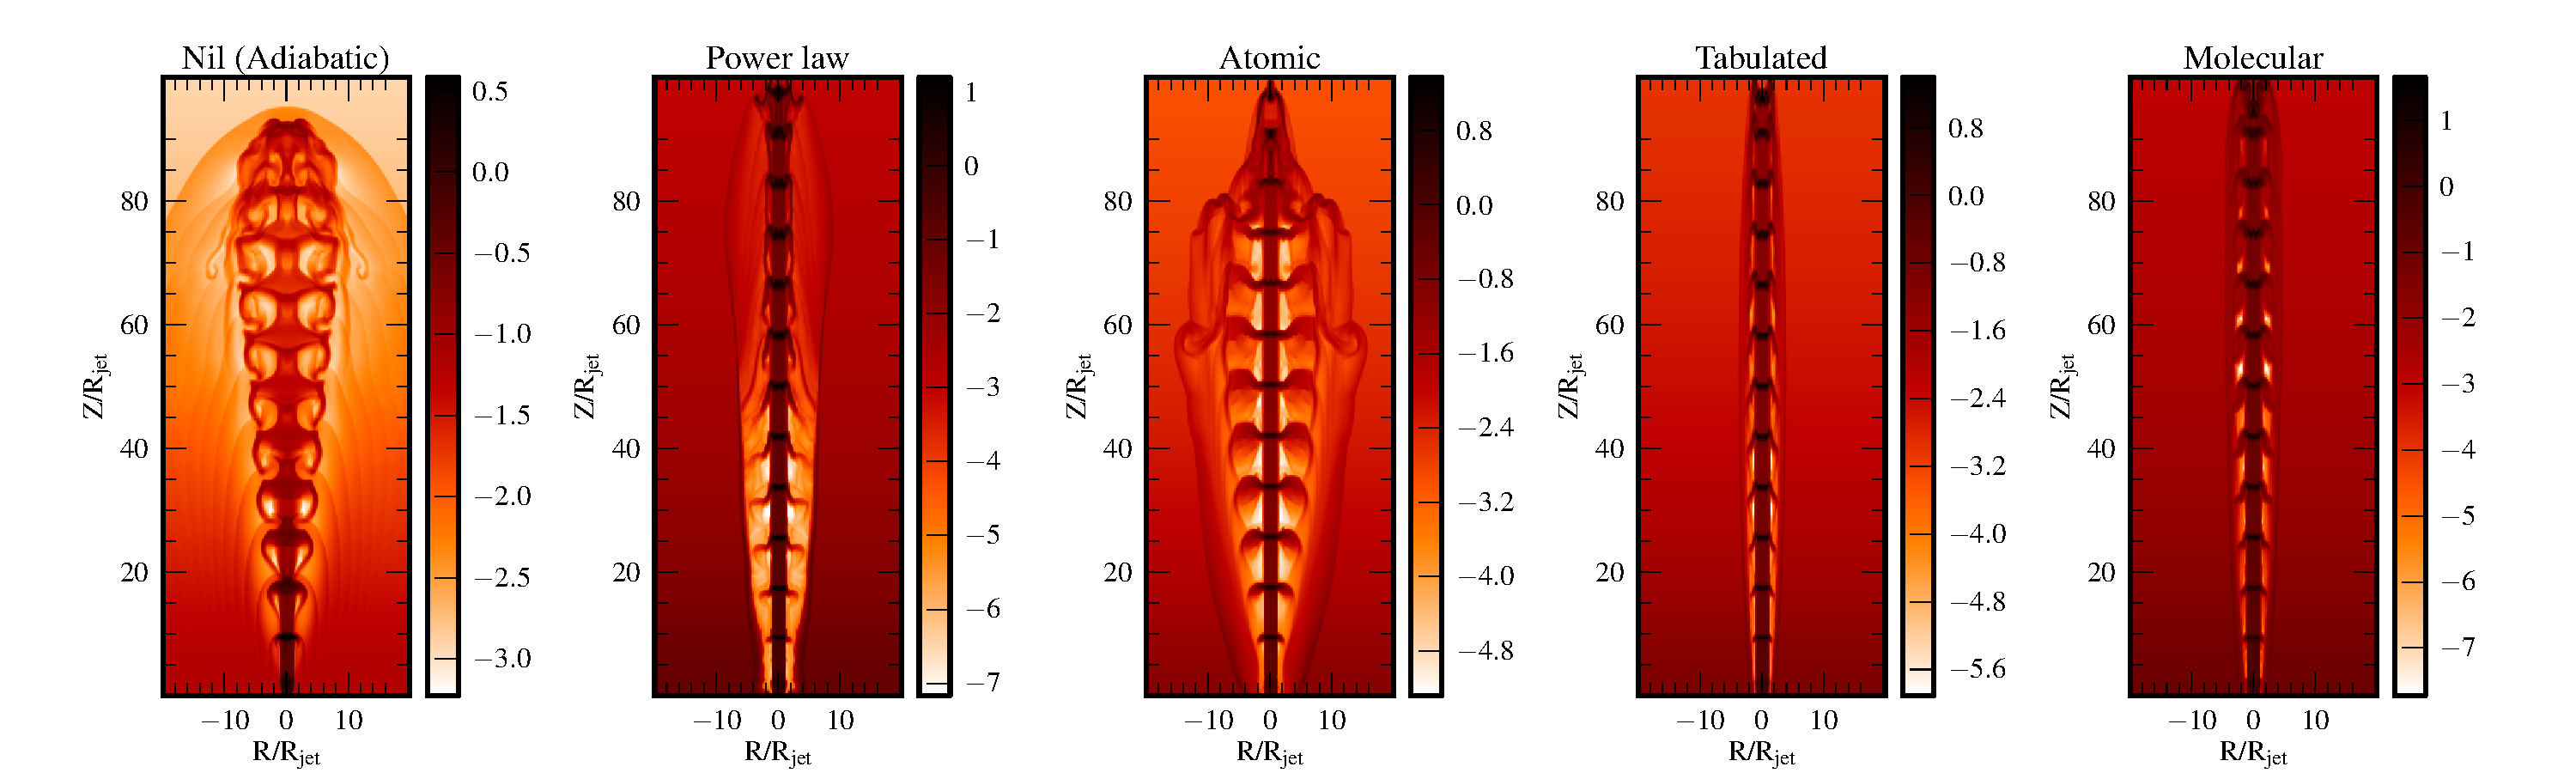
\includegraphics[width=2.\columnwidth]{\figpath/diffcool_sim.pdf}%{\figpath/jetplt1_1010.png}
 \caption{Jet Volume Density for different cooling modes with
   $\eta$ = 10.}
\label{fig:coolcmpdyn}
\end{figure*}

\begin{figure*}
 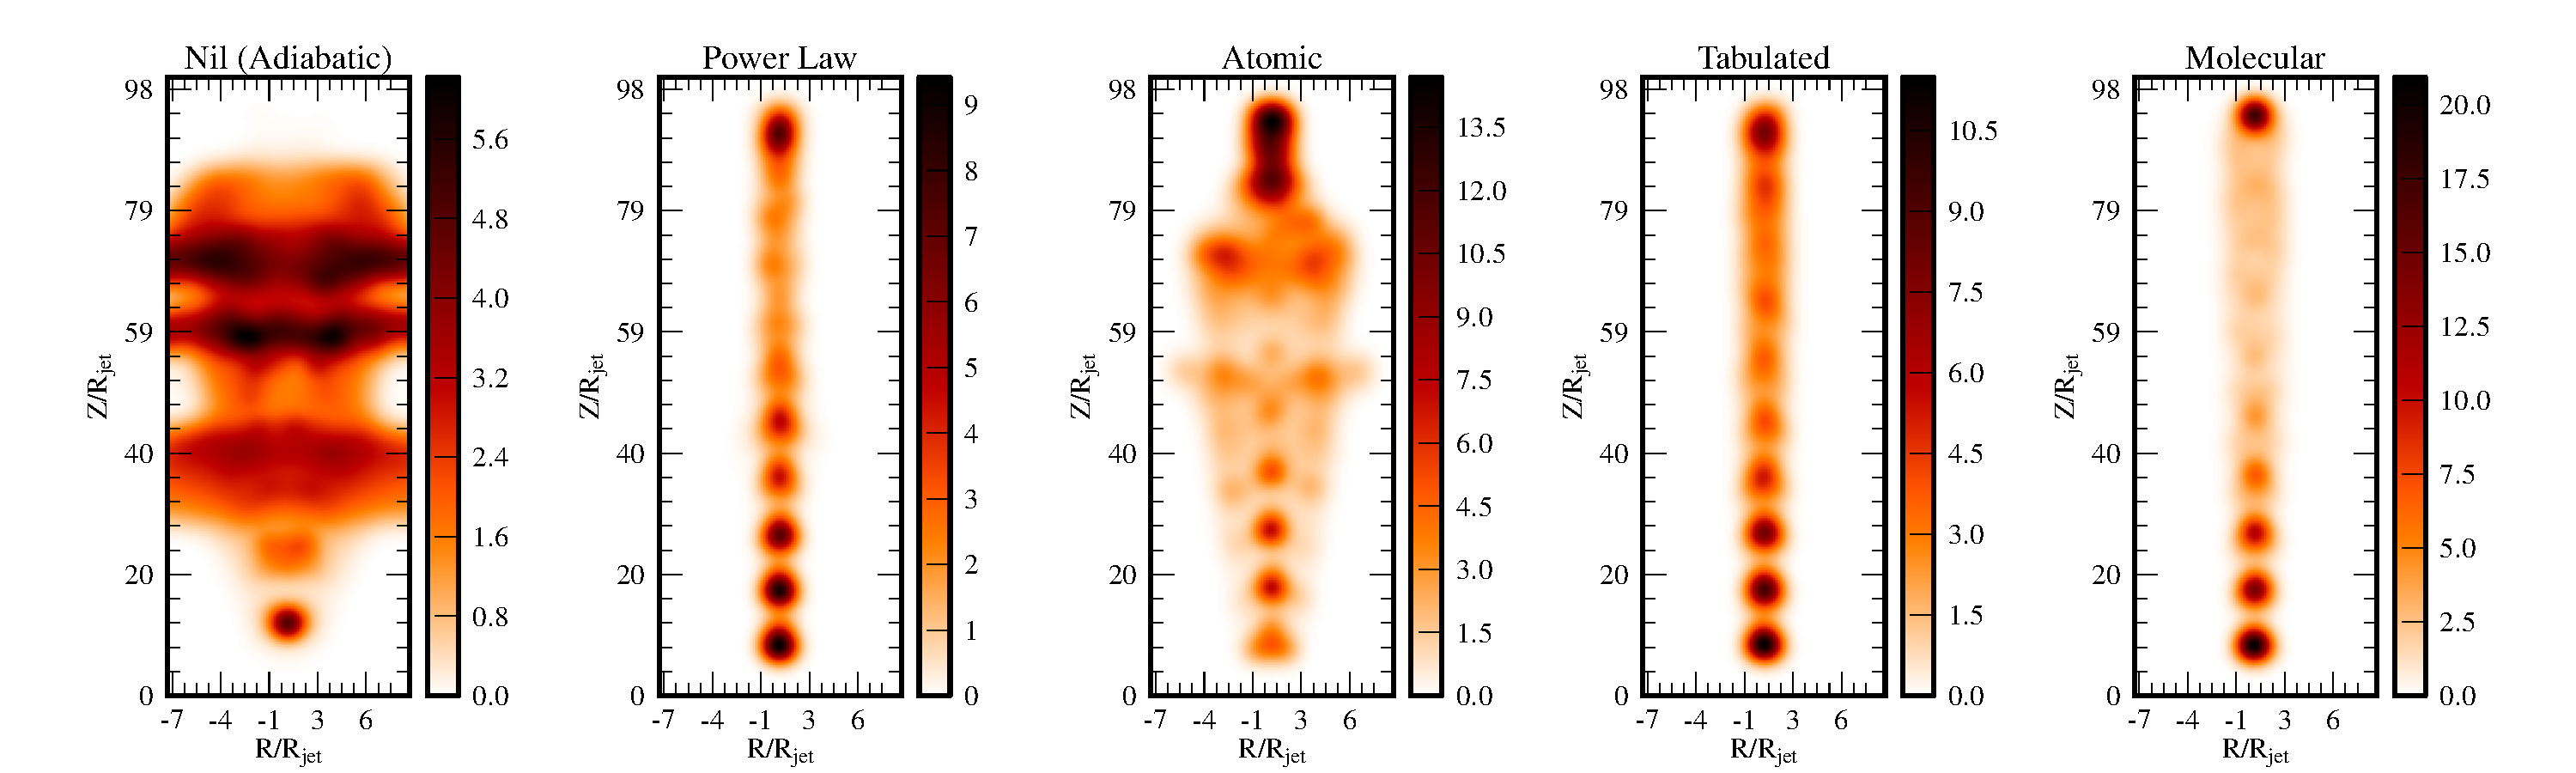
\includegraphics[width=2.\columnwidth]{\figpath/diffcool_img.pdf}
 \caption{A plot of the integrated SiO J=2-$>$1 emission from 5 models, 
each using a different method to calculate cooling and all with $\eta$=10.}
\label{fig:coolcmpsio} 
\end{figure*}


\subsection{Molecular cooling and H$_2$ Chemistry}
The molecular cooling in our
model includes the evolution of H$_2$ chemistry along with
contributions to cooling from fixed fractions of other molecules like
CO, OH etc. Figure~\ref{fig:Hfracsim} shows the color composite image
of various hydrogen fractions, (fHI (red), fH2 (green) and fHII
(blue)), from the dynamical simulation with
reference parameters. The jet beam is largely dominated by atomic
hydrogen, while molecular hydrogen is seen to be formed in internal
knots and region that is thermally instable. 
Ionized hydrogen is mainly formed at the tip of the bow. 
The highest temperature of $\sim$ 50000\,K is attained in our flow at the
tip of the bow shock. While the temperature on the edges (i.e.,interface between
jet and the ambient medium) is lower than 5000\,K. Also the relatively
weaker shocks formed nearby knots do not heat up the material beyond
10$^{3}$\, K. 
%

\begin{figure}
 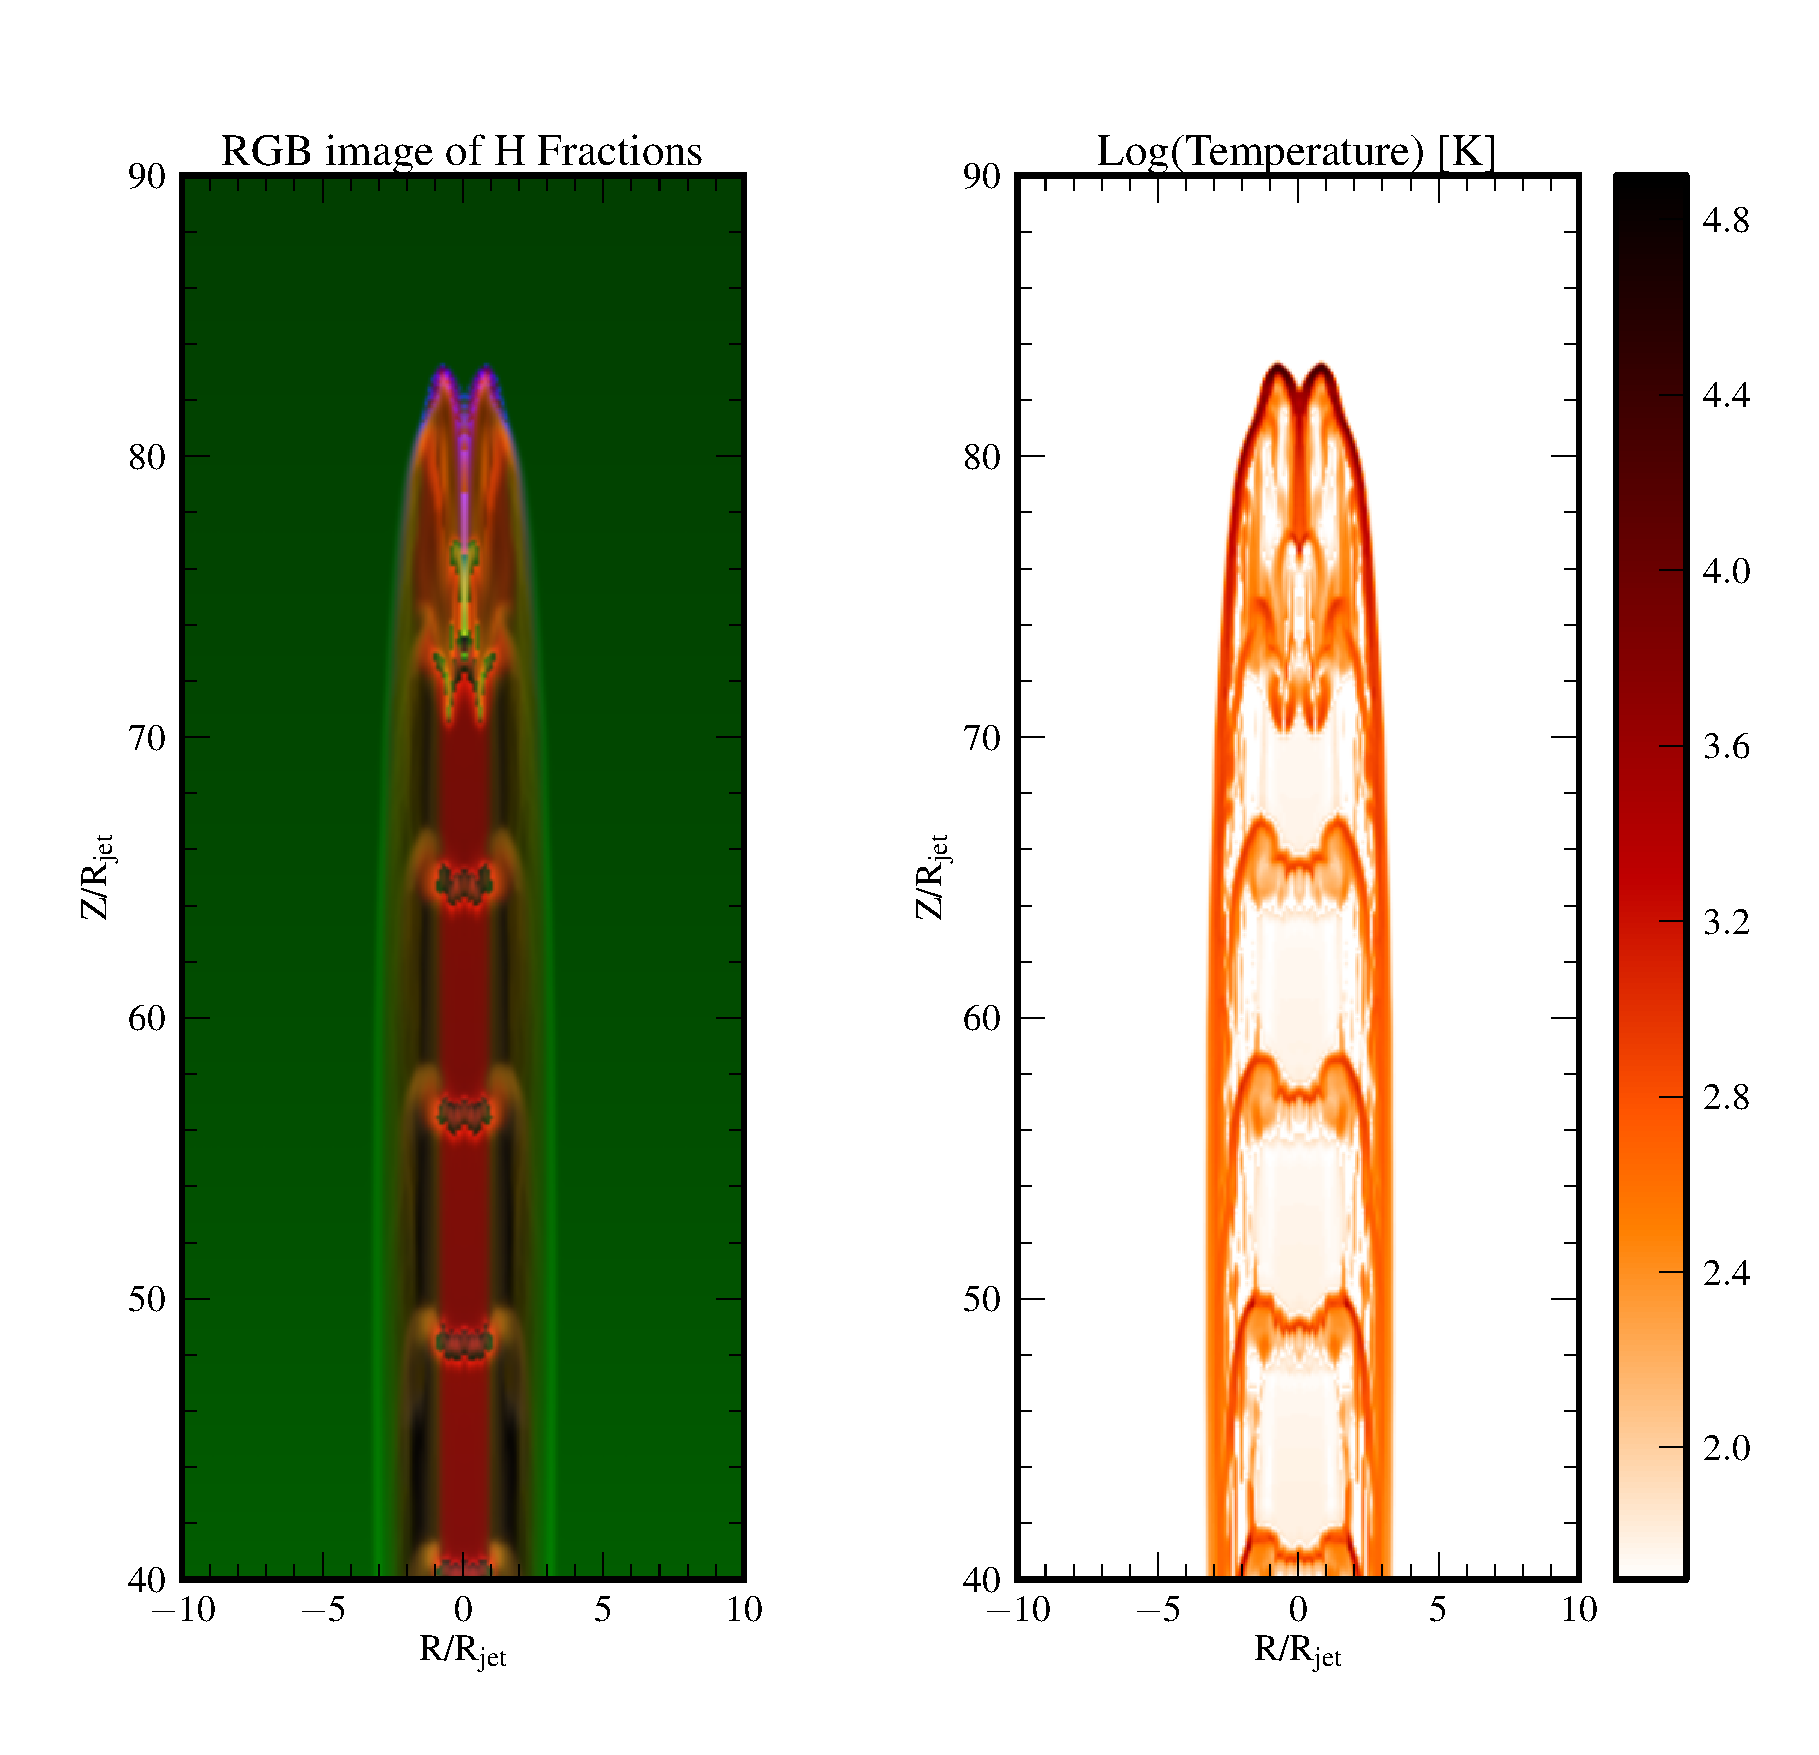
\includegraphics[width=1.\columnwidth]{\figpath/hfracs_ref.pdf}
 \caption{{\it{Left}} Color composite image of various hydrogen
   fractions, fHI (red), fH$_{2}$ (green) and fHII (blue), for the
   reference run. For better visualisation, the ionized hydrogen
   fraction is enhanced by a factor of 100. The temperature of the jet
 obtained from dynamical simulation is shown on the {\it{right}}.}
\label{fig:Hfracsim}
\end{figure}


The distribution of fractions of different hydrogen species along with
temperature suggests that there are essentially three regions where
chemistry is evolved due to shocks.
They are : (1) The tip of the jet , (2) The edges of the jet and
(3) intermediate knots. 
As the atomic jet propagates from the lower boundary 
into the cold molecular medium , it forms a strong shock resulting in
forming a density and temperature discontinuity. Such a jump in
dynamical quantities plays a crucial role in the evolution of
chemistry. For example, temperatures beyond few 1000\,K produced in the shocks could
disassociate the molecules and can also lead to ionization if
the temperature becomes larger than 10$^{4}$\,K.
%
\begin{figure*}
 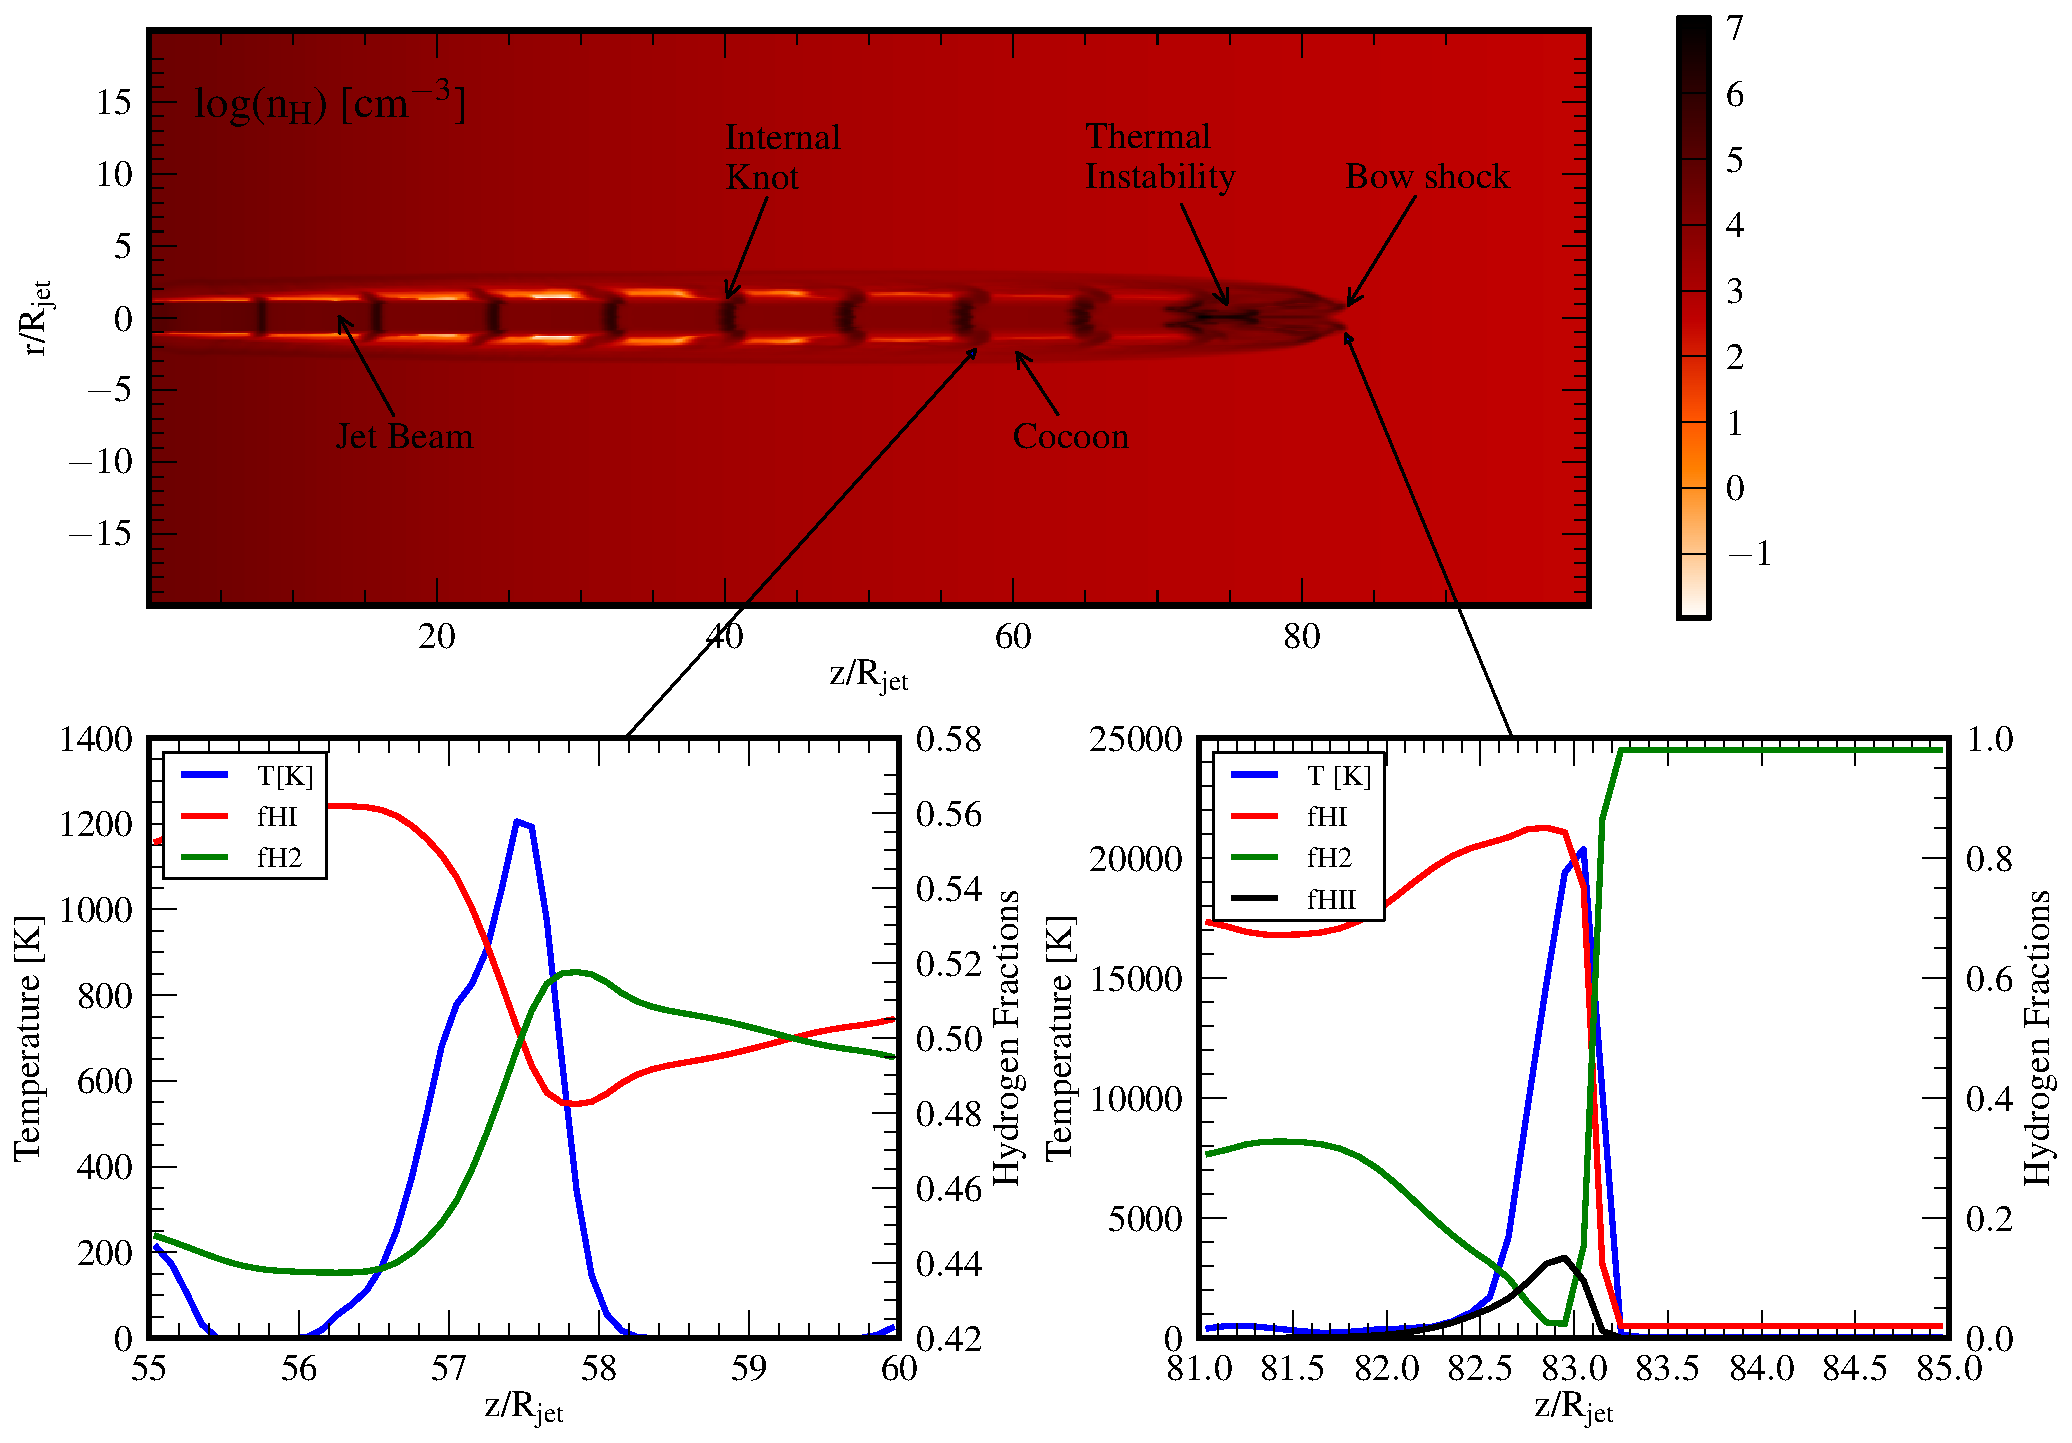
\includegraphics[width=2.\columnwidth]{\figpath/molcjet_310_molform.pdf}
 \caption{Dependence of hydrogen fractions on the temperature at two
   points in the flow, viz. the interface of the knot with molecular
   medium and at the bow shock.}
\label{fig:Hmolform}
\end{figure*}

For the reference run, the effect of the shock in the dynamical evolution of
the hydrogen fraction is presented in figure~\ref{fig:Hmolform}. The top
panel of the figure shows the hydrogen number density in the jet. 
The fraction of all hydrogen forms are shown in bottom
panels of figure~\ref{fig:Hmolform} along two representative regions in
the jet marked with the arrows. The left bottom panel shows the
vertical distribution of temperature, molecular and atomic fraction at the
interface of the knot and the ambient medium. The interaction of the
knot with the medium raises that temperature to 1200\,K and
accumulates the matter so that the density increases up to
10$^{6}$ cm$^{-3}$. Behind the shock as the material cools, atoms
combine together to form molecules as seen in the increase of fH2 from
0.44 to 0.52. Further away from the
shock, atomic and molecular hydrogen tend to reach a quasi equilibrium as their
fractions reach a value of 0.5. The ionized fraction is
extremely low in this region due to low temperatures. However at the
bow-shock, temperatures rise up to 20000\,K. Molecular
hydrogen species are destroyed, while ionized hydrogen shows an
increase in its fraction 
(figure~\ref{fig:Hmolform}). The peak in ionized fraction of 0.15
coincides with the peak in temperature profile as expected. The
molecular fraction shows a considerable dip from 0.3 to 0.03 at 
this temperature before rising sharply in the ambient molecular
medium. 
%

\subsection{Emission Maps, Spectra and PV diagrams}
\label{ssec:emspecpv}
The output obtained from the radiative transfer calculation is a data
cube with velocity being the third axis. This allows us to obtain
spectra and position velocity diagrams from these data cubes. 
Figure~\ref{empvspec90} shows outputs from the data
cube for SiO(2-1) in the reference run. 
The top left panel in the figure shows the emission map for the jet
directed downwards. The notable features are the knots close to the
base of the jet and the emission near the bow shock due to density
enhancement by cooling instability. The PV diagram shown in the top
right panel is obtained along the jet as indicated by the vertical magenta
line in the left panel. The velocities are show along the X-axis. High velocity features
are clearly seen in regions corresponding to the knots in the emission
maps. These features fade along the jet as the knots also disappear in
the emission map. The region close to the bow shock also shows high
velocity features.
%

\begin{figure}
 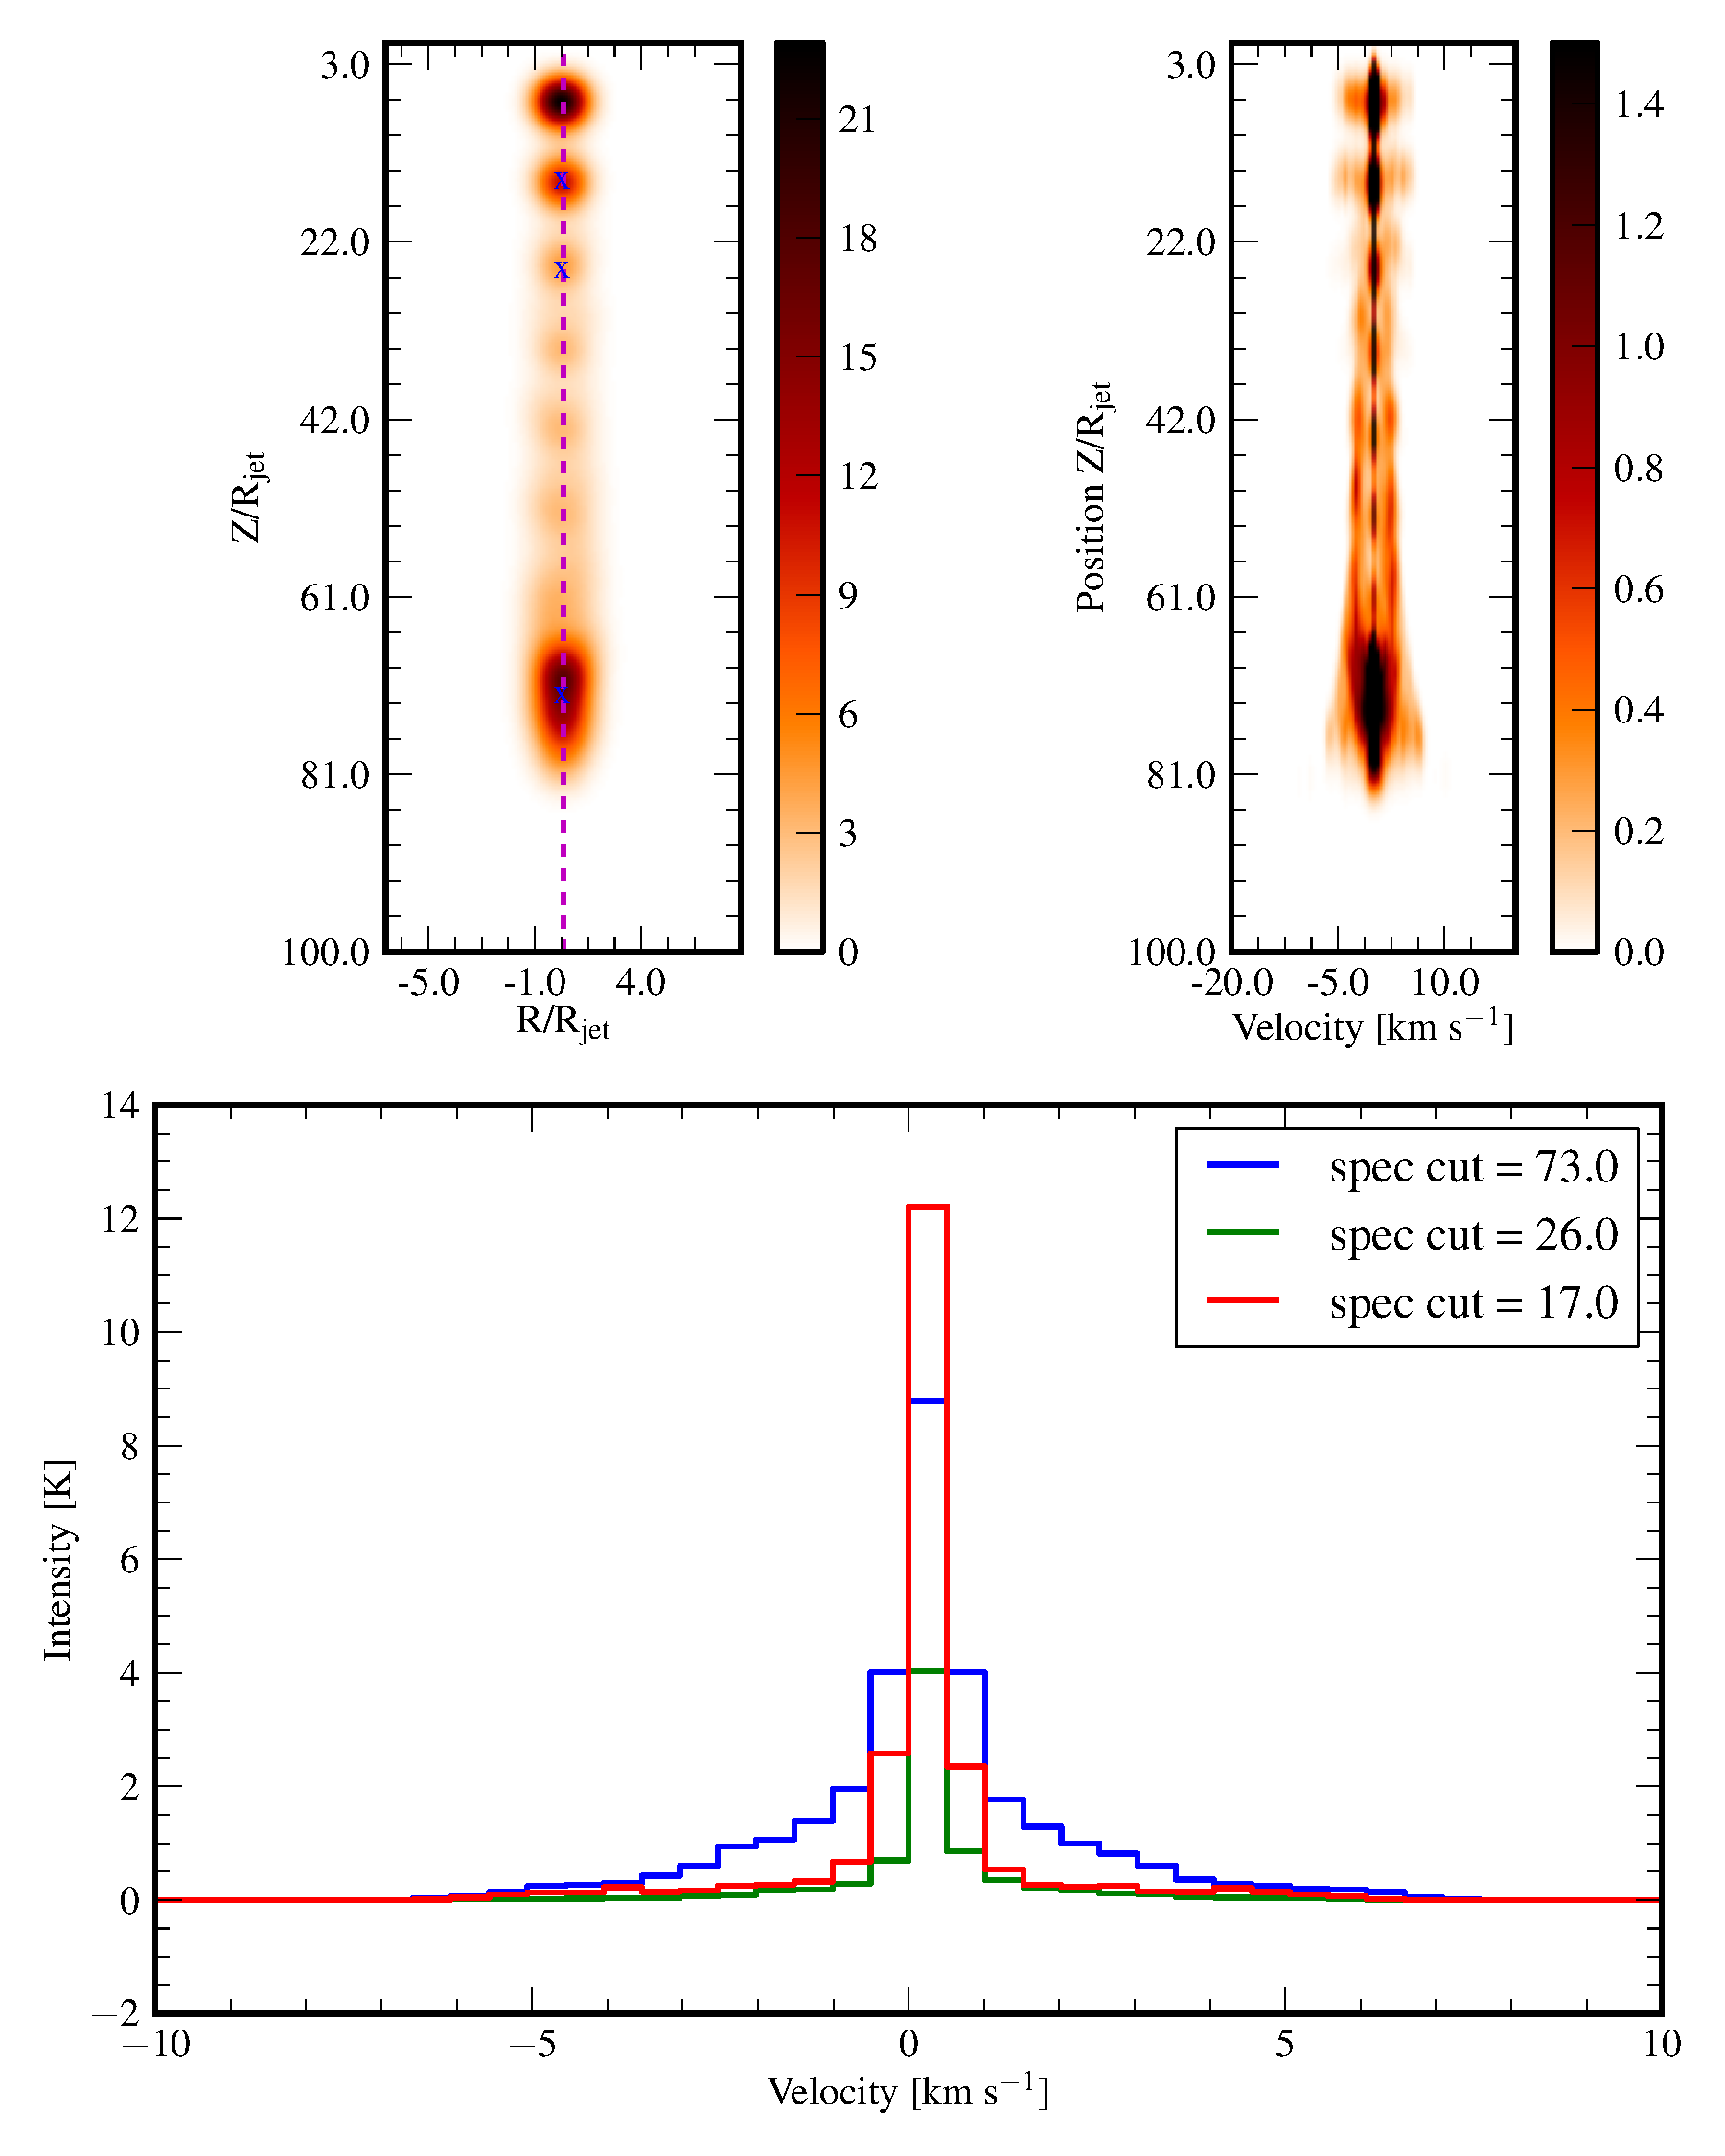
\includegraphics[width=1.\columnwidth]{\figpath/emspecpv_90.pdf}%{\figpath/refrun_21_90_emspecpv.png}
 \caption{Integrated emission map ({\it top left}), PV diagram ({\it top right}
   and spectra ({\it bottom}) for the
   2-$>$1 SiO transition for the reference run. 
   The jet is assumed to be in the plane of sky implying an angle of
   inclination of $90^{\circ}$. The vertical {\it magenta dashed} line
   represents the cut for the PV digram and green crosses marks the positions from which the spectra are taken.} 
\label{empvspec90}
\end{figure}

The spectra at three different positions in the flow are shown in the
bottom panel of figure~\ref{empvspec90} (they are marked with green
crosses in top left panel). The knot closer to the base is the brightest
showing a peak intensity of 25\,K. The
intensity decreases and reaches to about 10\,K close to the bow shock.
The line widths seen are typically around 5-10 km s$^{-1}$.
These line widths increase substantially as the angle of inclination
decreases. Figure \ref{empvspec45} show the
emission map, PV diagram and spectra for the same reference run but
with angle of inclination of 45$^{\circ}$
respectively. The line 
widths now are typically of the order of 20 km s$^{-1}$. 
The PV diagrams in these runs are not longer symmetric. Instead, they show a distinct {\it zig-zag}
pattern at each of the knots and region close to the bow shock.


% \begin{figure}
%  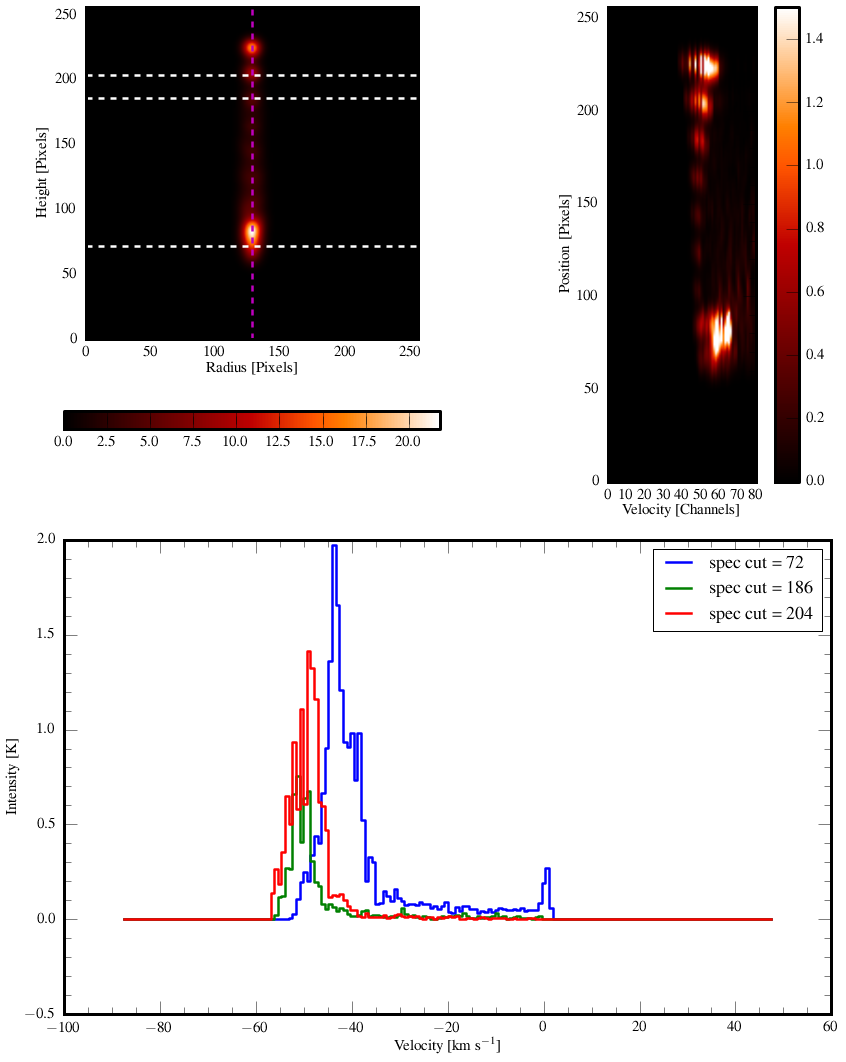
\includegraphics[width=1.\columnwidth]{\figpath/refrun_21_60_emspecpv.png}
%  \caption{Same as figure~\ref{empvspec90} but with angle of
%    inclination of $60^{\circ}$.} 
% \label{empvspec60}
% \end{figure}

\begin{figure}
 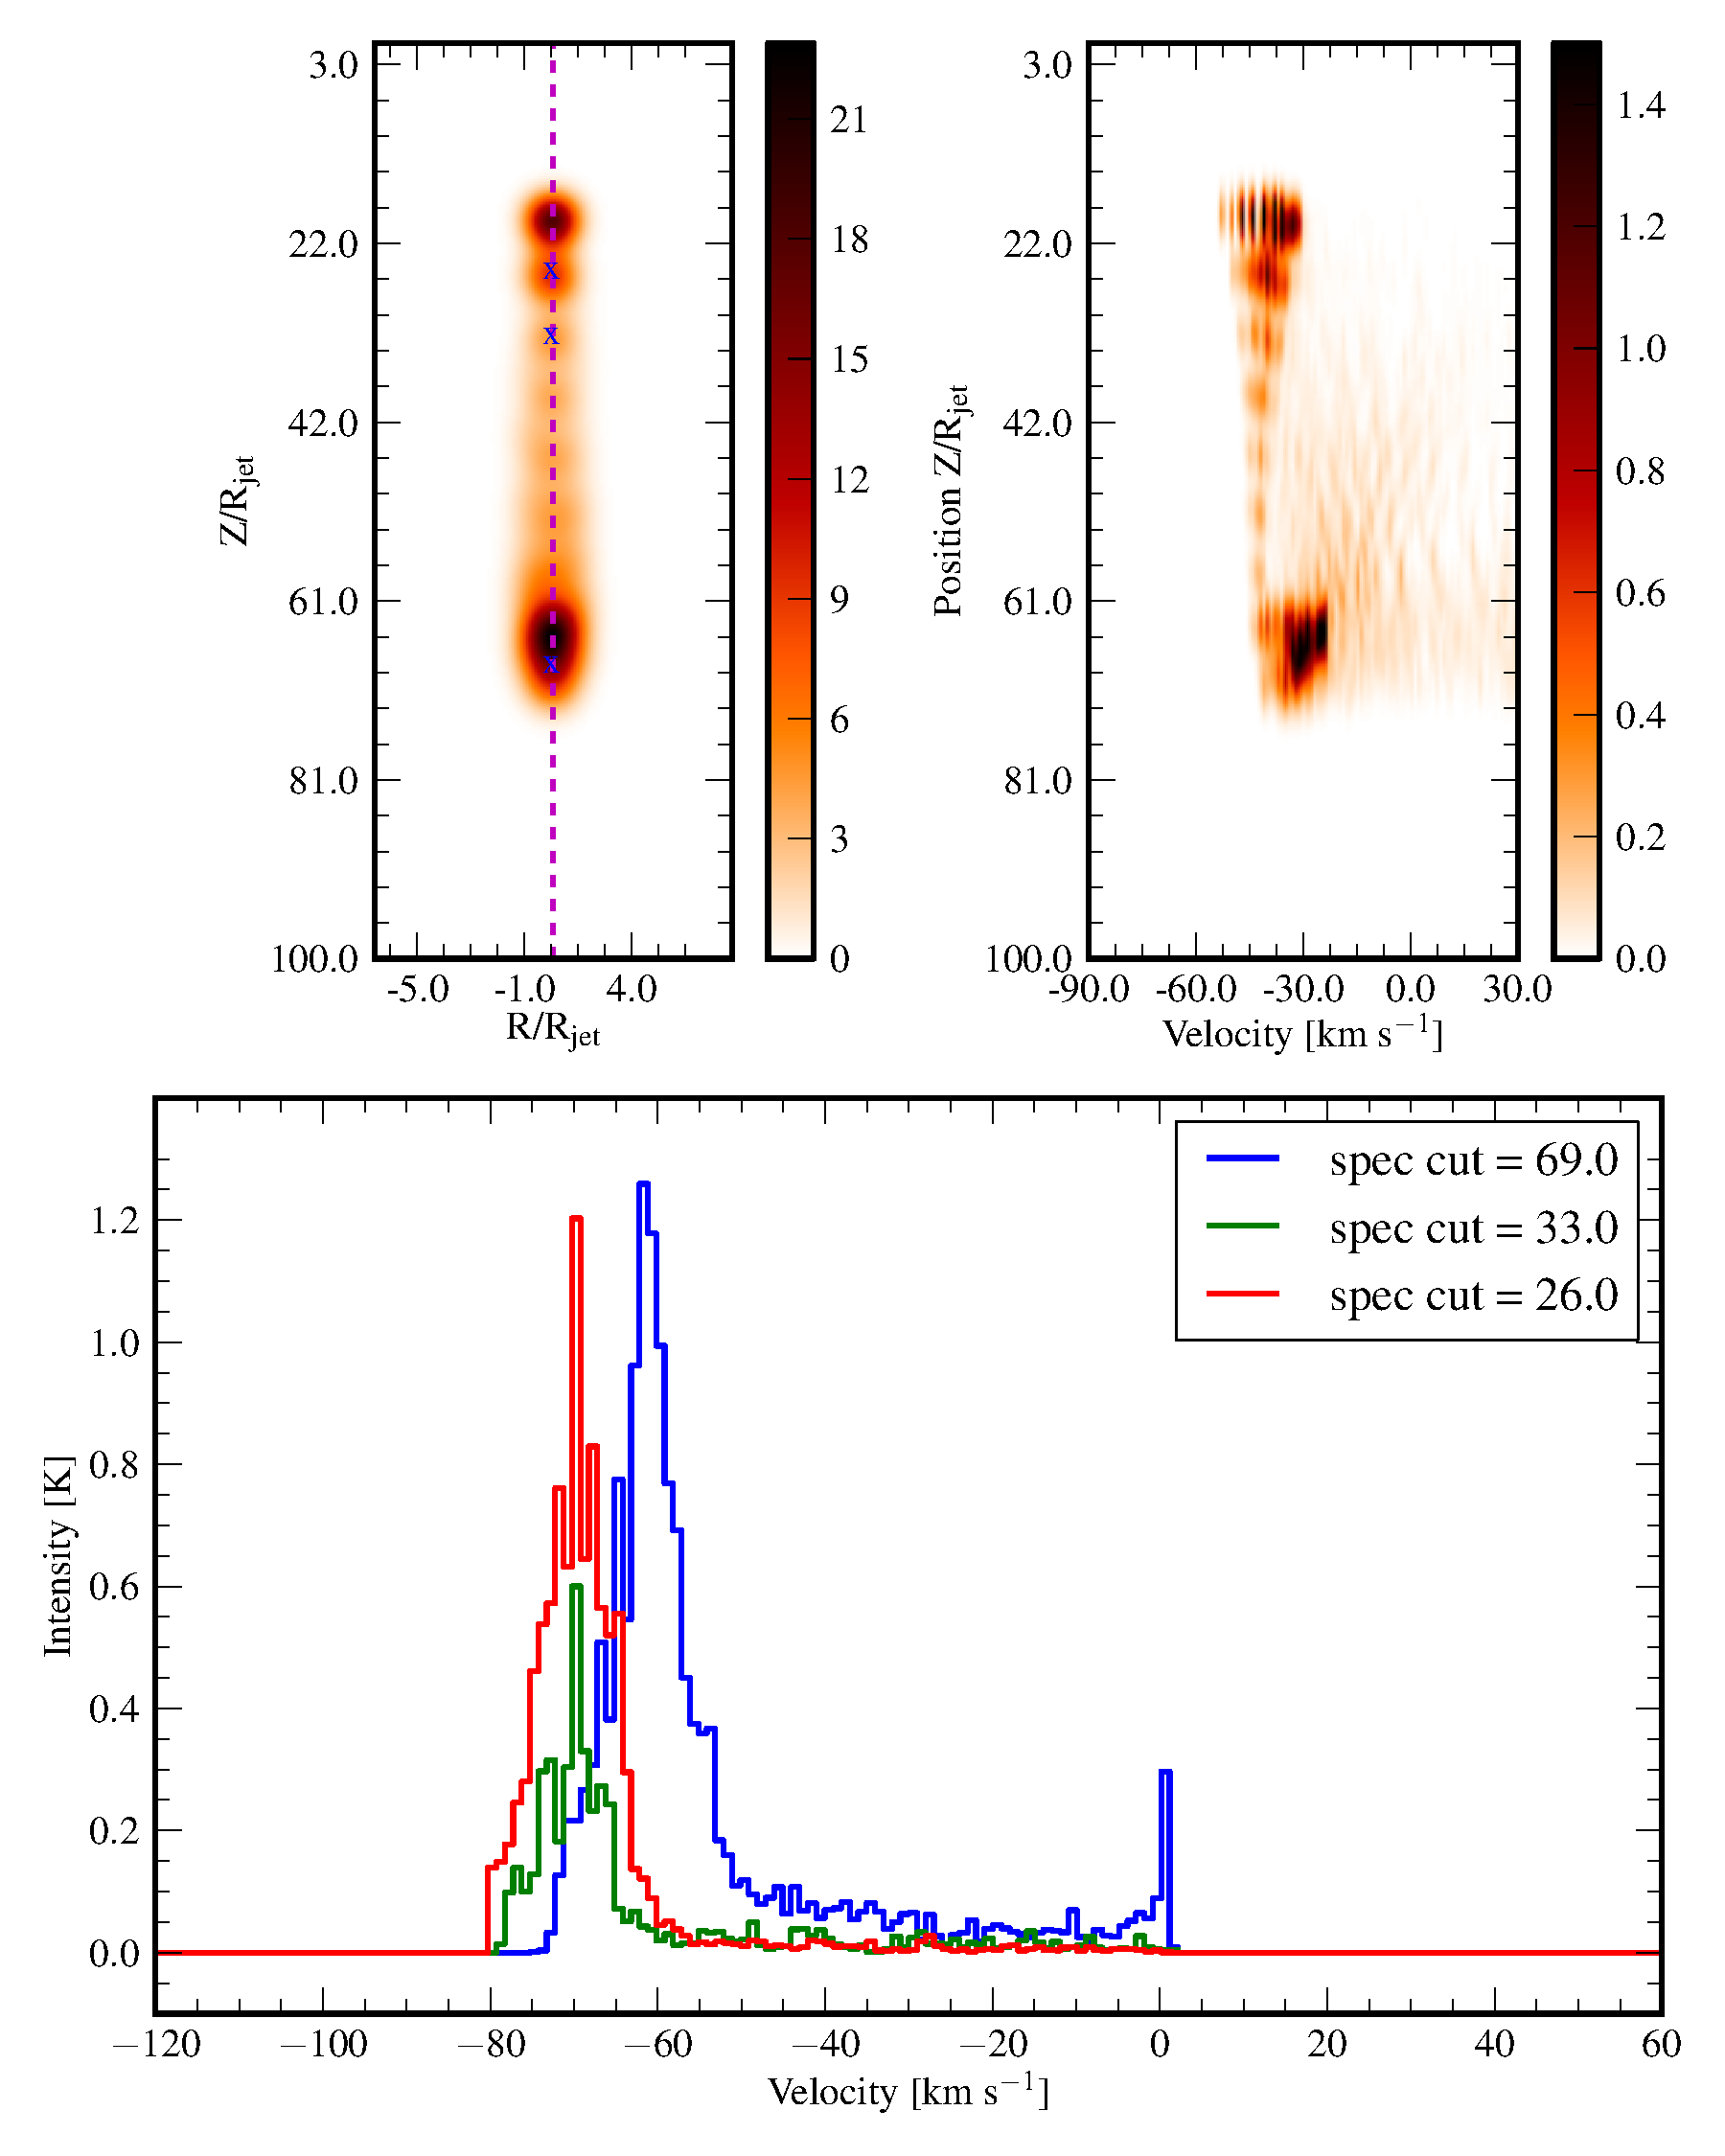
\includegraphics[width=1.\columnwidth]{\figpath/emspecpv_45.pdf}%{\figpath/refrun_21_45_emspecpv.png}
 \caption{Same as figure~\ref{empvspec90} but with angle of
   inclination of $45^{\circ}$.} 
\label{empvspec45}
\end{figure}

% %
% The predicted emission maps, spectra and PV diagrams are shown above to depend
% on the angle of inclination. In the next section, we focus on the
% dependence of these observational features on the 
% different fractional abundance profiles of SiO.



\subsection{SiO Abundance profile}
\label{ssec:sioabunem}
The fractional abundance of SiO has been assumed to vary with shock velocity in
a simplistic manner (see sec~\ref{ssec:sioabun}). In
figure~\ref{fig:diffabunem}, we compare the maps for J = 2-$>$1
emission at an inclination angle of 90$^{\circ}$ for three different abundance profiles and two different ratios of shock to
jet velocities, $\delta$. There is a striking difference with regards to
emission from the internal knots in these images. Using the top hat profile
and accounting for shock speeds (i.e. $\delta < 1$) results in
emission from  all the internal knots in the J=2-$>$1 line. However, some of
these knots are not observed when using the same top-hat profile but
assuming the shock velocity to be same as the jet velocity (i.e.,
$\delta$ = 1). Similar qualitative characteristics are seen in case of a gaussian
abundance profile. In particular, the case with $\delta$ = 1 only
produces emission from the knot closest to the bow shock, while the internal
knots do not show any appreciable emission. The step function and
gaussian step (not shown) with $\delta = 1$ produces very similar
features as that of the top hat profile with $\delta < 1$.
Further, the emission from
the knot closer to the bow shock varies considerably with different
profiles and value of $\delta$. It is the brightest for the case with
a top-hat profile and $\delta < 1$. The peak emission and line widths at this knot
are listed in table~\ref{tab:result2}.
%

\begin{figure*}
 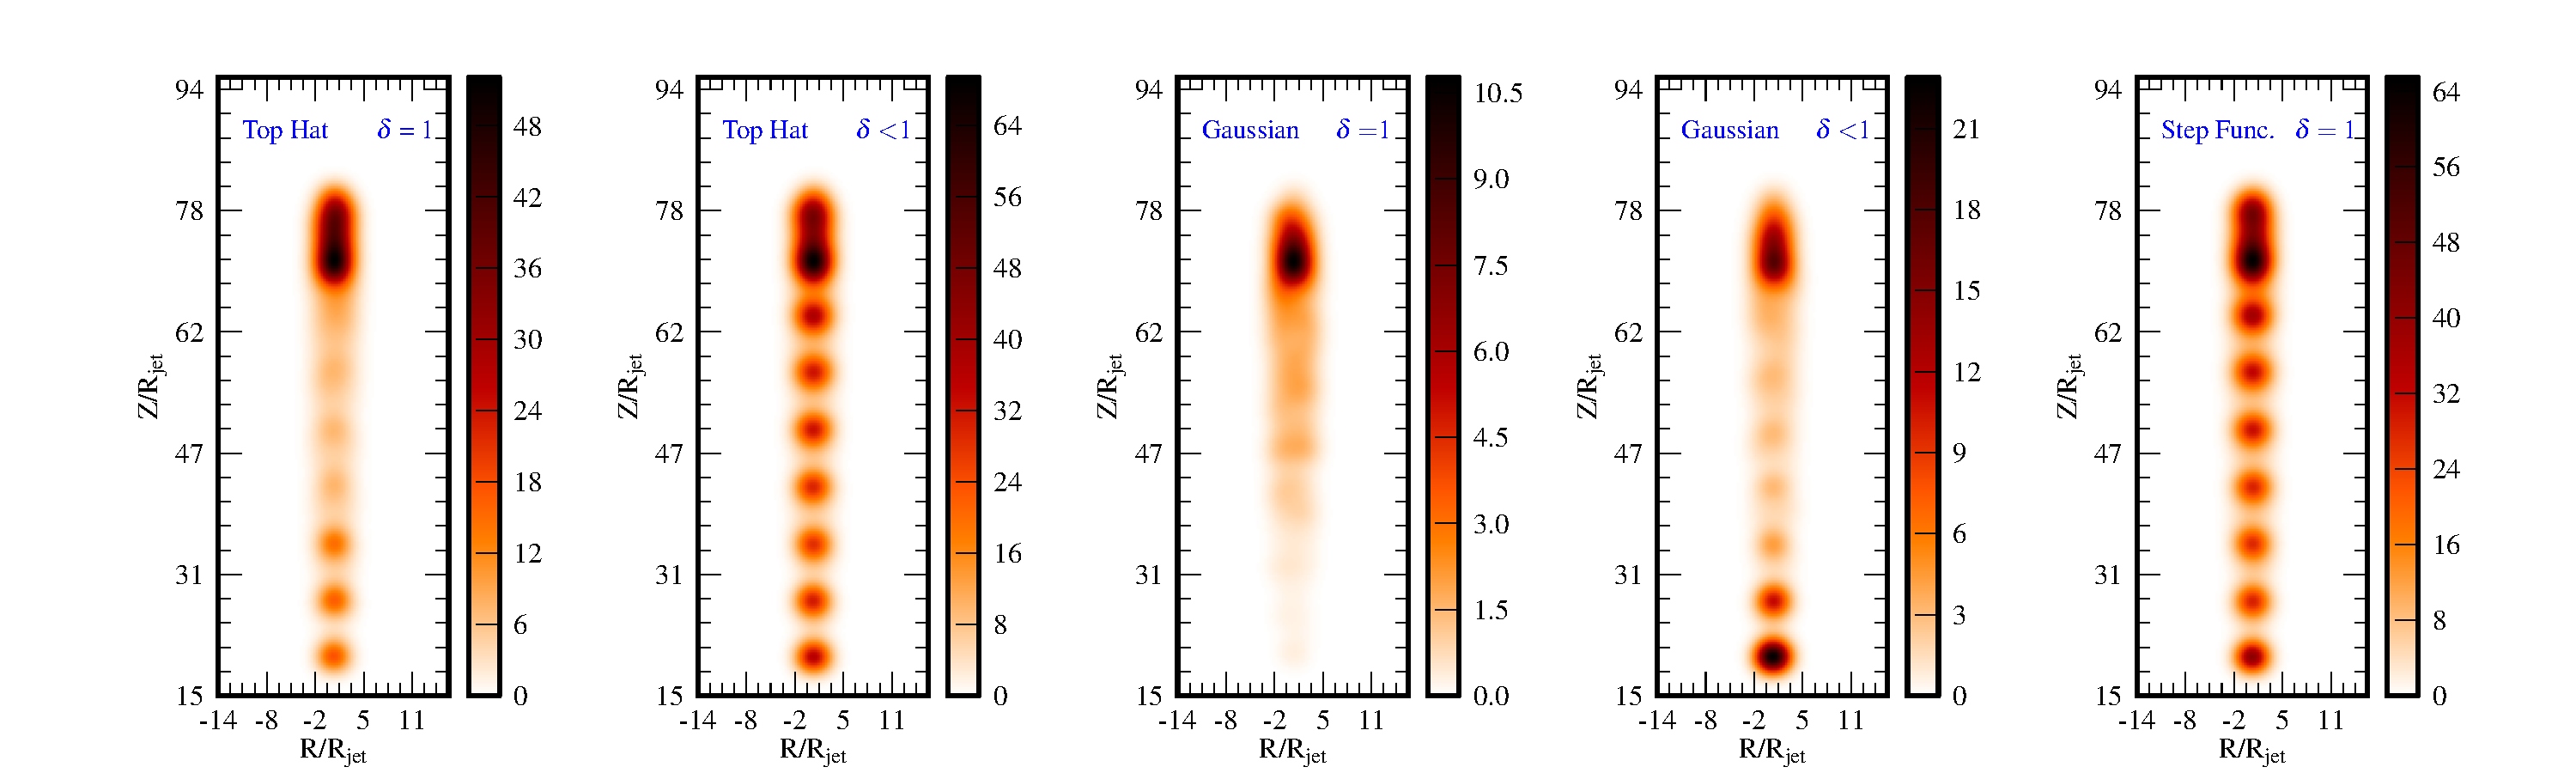
\includegraphics[width=2.\columnwidth]{\figpath/diffabun_img.pdf}%{\figpath/EM_gaussandth.png}
 \caption{Variation of 2-$>$1 SiO emission for runs with molecular
   cooling having different abundance profiles.}
\label{fig:diffabunem}
\end{figure*}


The dependence of emission on SiO abundance profile is expected due to
the distribution of jet velocity obtained from dynamical
simulations. We see that the velocity of internal knots lie around
70-90\,km\,s$^{-1}$, while the pulsed jet was injected with a mean of
100\,km\,s$^{-1}$. The knots slow down during the evolutionary
phase as they interact with the ambient medium. Interestingly, younger
knots closer to the base of the jet are brighter compared to older
ones further away from the jet (see panels 1 and 3 of
fig~\ref{fig:diffabunem}). This is attributed to the fact that the
ambient medium has a density gradient that goes as $\sim
z^{-2}$. Thus, the younger knots suffer the most deceleration closer
to the base of flow. This fact is taken into account when the shock
velocity is consistently calculated using the density contrast and
using a value of $\delta <$ 1. This process is further validated by
the lack of emission from internal knots in panel 3 of the
fig~\ref{fig:diffabunem}. 
%

Additionally, the internal knots show their distinct signatures in
form of {\em Hubble wedges} as seen in the PV diagrams for these
different profiles (see
~\ref{ssec:emspecpv}). Figure~\ref{fig:pvdiffabun} shows a zoomed in
version of the bottom four internal knots in form of a PV diagram for these
different abundance profiles. As expected, the signatures of knots 
is missing for the case with gaussian profile with $\delta$ =
1. Further, the wedges formed in panels 1, 2 and 5 of the figure in
general are slightly more extended as compared to those
formed in panel 4. This is indeed because of the
discontinuous nature of the top-hat abundance profile as the SiO is
enhanced to a maximum abundance for all velocities between 20 and 100
km\,s$^{-1}$, which is not the case in a more continuous gaussian
distribution.

\begin{figure*}
 \includegraphics[width=2.\columnwidth]{\figpath/diffabun_PV.pdf}%{\figpath/PV_gaussandth.png}
 \caption{Position-velocity maps of SiO(2-1) for the internal
   knots produced in the model with reference parameters and different abundance
   profiles. The contours mark different levels of emission in Kelvins, viz.,
   0.2,0.6,1.0,1.4,1.8,2.0,3.0,4.0.}
\label{fig:pvdiffabun}
\end{figure*}
   
 
\section{ALMA view}
\label{sec:ALMAview}
%
In order to see the interior structure of the molecular outflow and
test the model predictions, high
resolution interferometric observations are needed. 
We have performed synthetic Atacama Large Millimeter
Array (ALMA) observations using the Common Astronomy Software
Applications package (CASA). The output from the radiative transfer
were scaled to a distance of 300pc and used as the sky models for observations of
the J=2-1, J=5-4 and J=8-7 lines at frequencies of 86.85, 217.10 and
347.33$\,$GHz, which fall in ALMA bands 3, 6 and 7, respectively. The observations
were simulated using cycle 1 ALMA for 30 minutes total integration
time, in the configurations c32-6, c32-4 and c32-3 for the three
lines, giving beam sizes of 0.72'', 0.47'' and 0.58'' and
sensitivities of 0.05, 0.07 and 0.09$\,$mJy/beam for the three lines
(as calculated by the ALMA online sensitivity calculator) with
velocity resolutions of $\sim$1$\,$km/s.
 Figure~\ref{fig:almafig}
presents the ALMA prediction obtained from our reference run. The
left panel shows the integrated emission of SiO J = 2-1 line while the right
shows the PV diagram for the same line and over laid are
the contours of SiO J = 5-4 and J = 8-7. The contour levels are marked
on the color bar of each panel. 


\begin{figure*}
 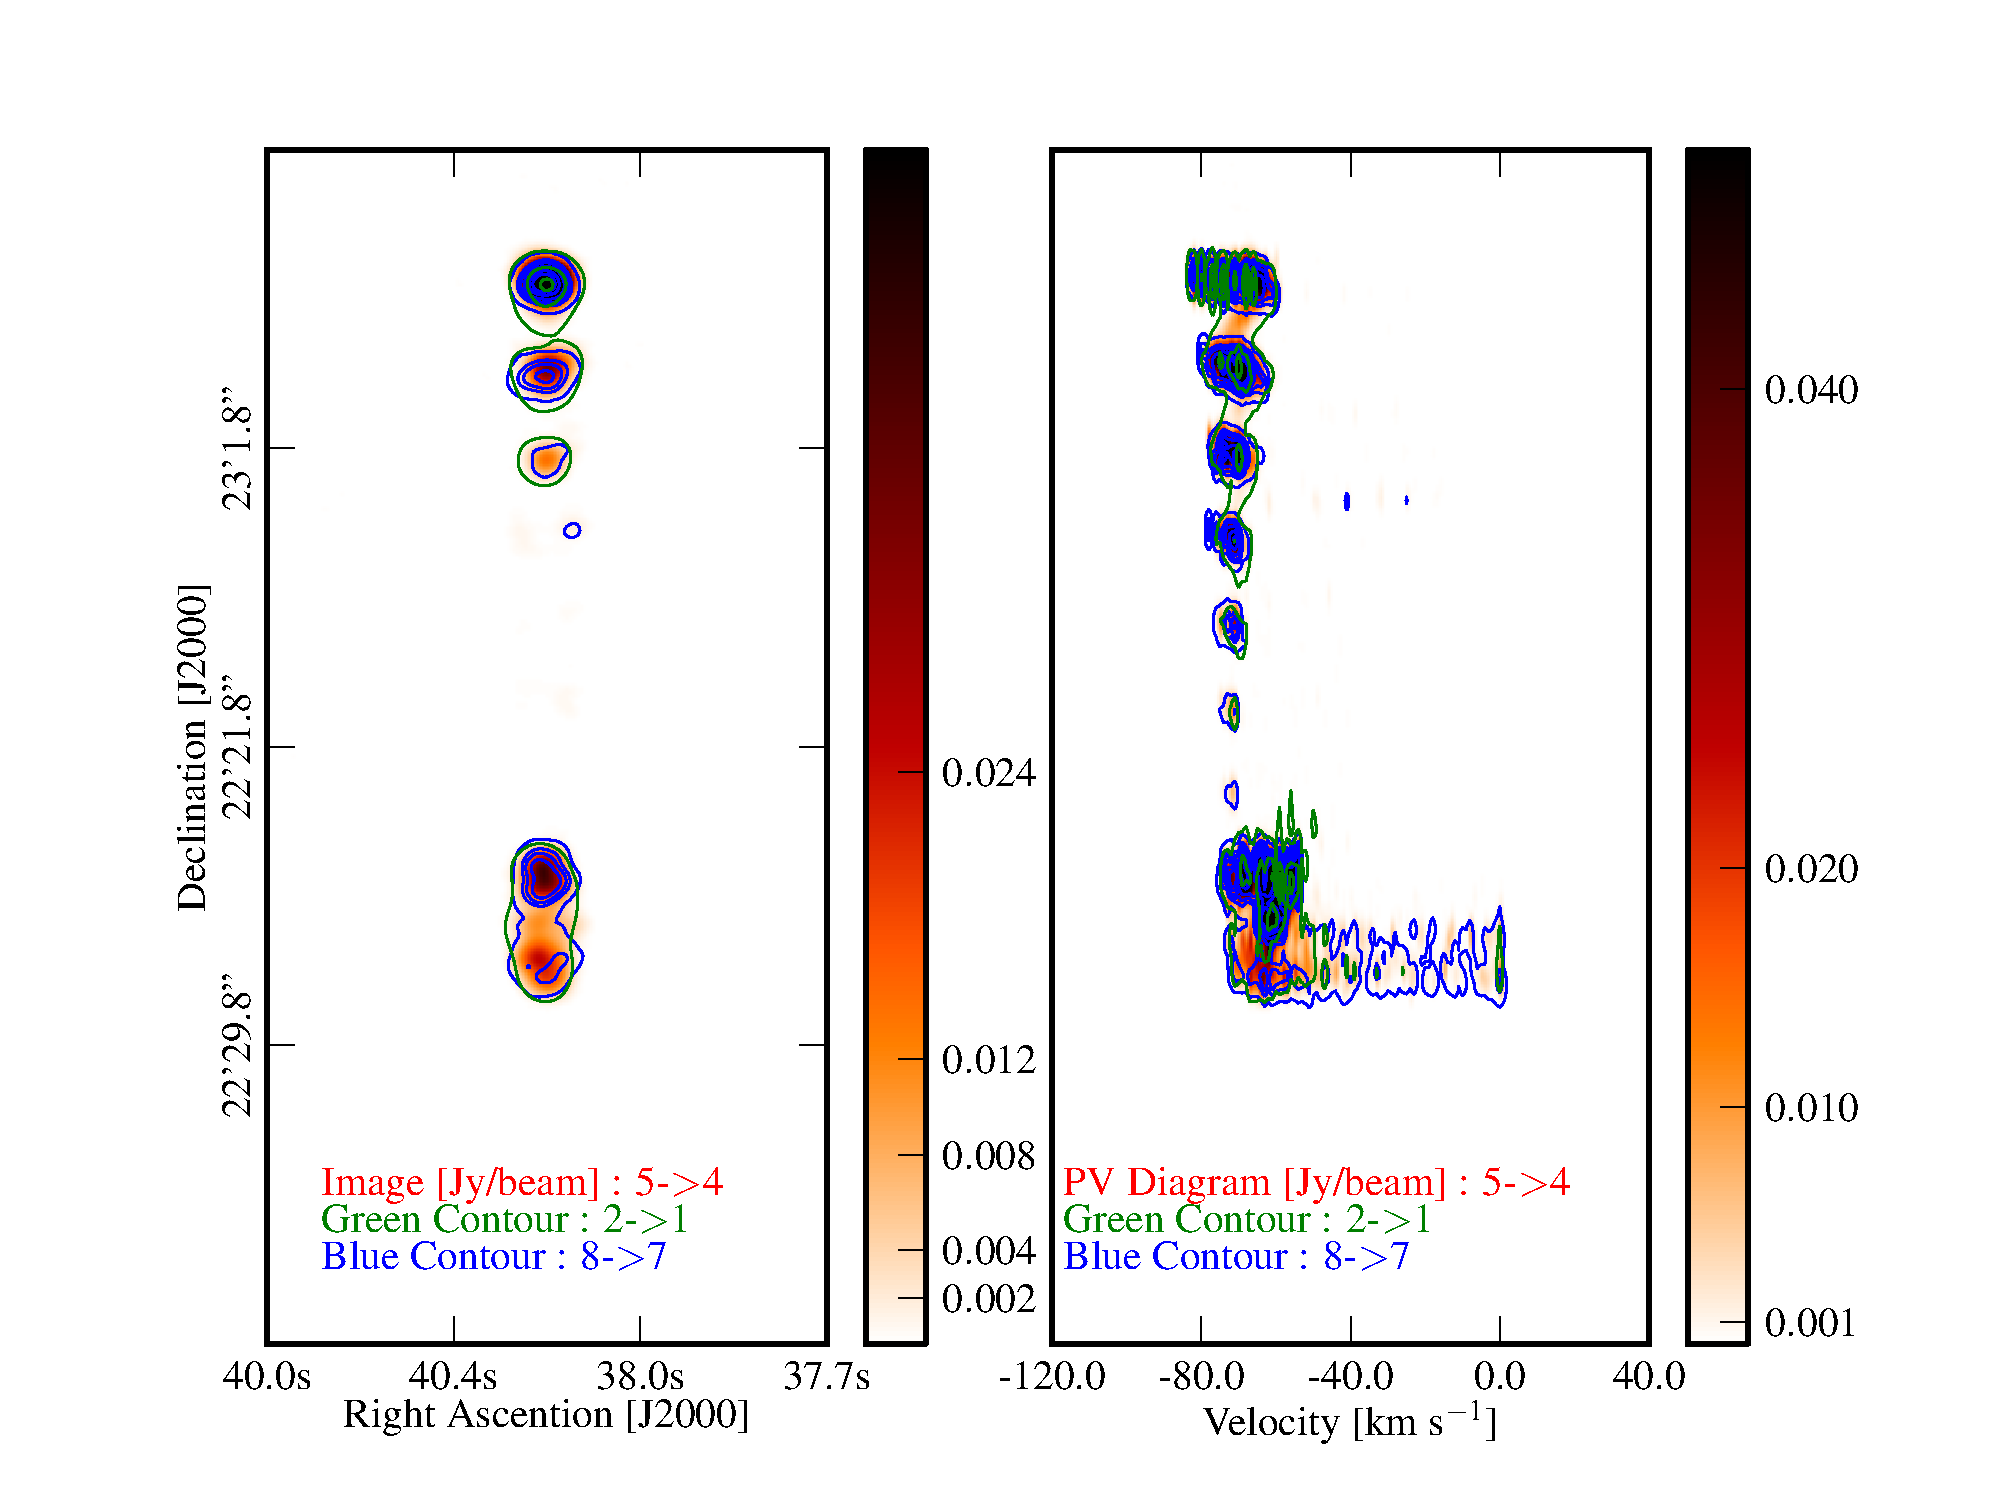
\includegraphics[width=2.\columnwidth]{\figpath/almamaps_new.pdf}%{\figpath/ALMAmaps3.png}
 \caption{{\bf Left:} The integrated intensity map of SiO(2-1), (5-4)
   and (8-7). The emission map shows the 5-4 line intensity (in units
   of Jy$\,$kms$^{-1}$/beam), the blue contours show the J=8-7 line
   intensity and the green contours show the J=2-1 line intensity. The
   jet is inclined at an angle of 60$^{\circ}${\bf Right:} The PV
   diagram taken along the axis of the jet for the 5-4 line (in units
   of Jy/beam), showing the higher J transitions highlighting the
   knots of the jet and broad emission at the bow shock. 
   In both panels the ticks on the color bar represent the different contour levels.}
\label{fig:almafig}
\end{figure*} 

ALMA Cycle 0 observations have recently reported complex kinematic
features of young bipolar molecular outflows. In particular,
\cite{Arce:2013p14902} observed morphology, kinematics and entrainment 
of the HH 46/47 molecular outflow from a low mass nearby
source (d = 450 pc) using CO(1-0). They find that the red
lobe of the outflow exhibits a very complex structure with a
collimated episodic wind, whereas the outflow in the blue lobe is
consistent with a
wide-angle wind model. Three major clumps in the red lobe along the
outflow axis appear as {\em{wedges}} in the PV
diagram (similar to that seen in the right panel of fig~\ref{fig:almafig}). 
A quantitative comparison is not possible due to the different
molecule observed. Another source which is studied in details with ALMA band 7 is
one of the most energetic, luminous molecular outflows
G331.512-0.103 (\citealt{Merello:2013p15066}). Observations of this outflow
associated with a high mass star reveal a compact, extremely young
bipolar outflow and a symmetric outflowing shell. Further, their PV
diagrams with SiO and H$^{13}$CO$^{+}$ show a characteristic peak at
-45\,km\,s$^{-1}$ along the primary axis that could associated with a 
molecular {\em bullet} of high-velocity dense material as also found in our
synthetic maps at inclination angles of 60$^{\circ}$ and 45$^{\circ}$.

 
\section{Discussion}
\label{sec:discussion}
Here we compare our results with SiO observations of young low
mass and high mass outflows.

\subsection{EHV component and Molecular bullets}
\label{ssec:EHV}
Multiline mm-wavelength surveys of SiO emission towards a sample of molecular
outflows have shown that these outflows exhibit both low and high
velocity SiO emission possibly arising from two distinct regimes. The slow
component in the case of a typical outflow, L1448, is believed to arise from
the shell of accelerated ambient gas with SiO abundance
lower by two orders of magnitude than regions emitting the high
velocity component
\cite{Codella:1999p12584}. In addition, an interesting feature of EHV
gas is seen in many young molecular outflows. The origin of the EHV
component is still a mystery, however, recent high resolution
observations show that EHV gas is seen in
high density gas tracers (like CO and SiO) and the line have
intensities $\sim$ 0.1 K (\citealt{Tafalla:2010p14759}).
%

In IRAS 04166+2706, \cite{SantiagoGarcia:2009p13972} have shown 
that the EHV CO(2-1) emission is mapping a jet-like
feature that consists of a collection of
discrete peaks symmetrically placed on both outflow lobes. This symmetry
indicate that such EHV peaks might arise from events that took place
near the central source and have since propagated in the flow
\citep{Bachiller:1990p11196, Tafalla:2011p14051}. The dynamical 
model in conjunction with proper radiative transfer calculations presented here 
agrees very well with the above scenario. The {\em{bullets}} in our
work are injected into the flow in a sinusoidal manner along with a
collimated atomic jet. These pulsating ejections do interact with the medium
via shocks and exciting high velocity gas. Including the cooling associated with
molecules and the H$_{2}$ chemistry allows us to
consistently identify the regions where molecular hydrogen is formed
and disassociated (see fig.~\ref{fig:Hmolform}). The SiO emission that we
obtain from our radiative transfer calculations is associated with
regions slightly behind where the shocked H$_{2}$ gas is present
as observed in case of L1157 molecular outflow
\cite{Gueth:1998p14058}. A contour map of SiO
emission obtained from the reference run is shown in
figure~\ref{fig:ltconts}. Further, we find SiO emission coming from velocities 
of the order of 40-60 km\,s$^{-1}$ (see fig
~\ref{empvspec45}). Additionally, we see a distinct saw-tooth pattern
in the PV diagrams from our models (see figs. \ref{empvspec45} and
\ref{fig:almafig}). These predictions from our model very well
resembles the characteristic features of EHV SiO emission 
seen in the majority of the outflows \citep{SantiagoGarcia:2009p13972,
  Tafalla:2011p14051, Arce:2013p14902}.
%

All of the above striking similarities from observations of EHV gas
and synthetic spectra and PV diagrams gives a very formidable backing
to the idea that such an emission could arise due to shock interactions of
internal knots in the flow. 

\subsection{Line transitions and ratio}
Numerous molecular outflows with jet-like bullets have been
observationally studied till date. In particular, H7-11
\citep{Bachiller:1998p14725}, IRAS 04166+2706
\citep{SantiagoGarcia:2009p13972, Tafalla:2010p14759}, HH211 \citep{Nisini:2002p14418}
L1448 \citep{Bachiller:1991p14732,Nisini:2007p13128,
  Tafalla:2010p14759} and L1157 \citep{Nisini:2007p13128} have
shown clear signatures of the EHV component. Among them, L1448, HH211 and
L1157 have been studied in detail using an extensive multi-line
survey of SiO. Such a multi-frequency analysis helps to understand the dependence of
excitation conditions for these lines on velocity, based on existing shock
models.  
%

The most striking feature seen in the figure~\ref{fig:ltconts} is the progressive shift of
emitting region from the interface to internal knots with increase in
excitation energies of different lines. In particular, the lowest
transition J=1-$>$0 shows most of the emission coming from the
interface between the jet and ambient medium, along with emission from
the dense knots formed at the base of the flow. On the other hand, SiO (5-4) and (8-7) emission, 
is more concentrated in the inner jet regions and arise mainly from
the shocks due to internal knots. Such a trend in emission with excitation energies coming from different SiO line transitions
have been observed in young outflows (for e.g., {\it{L1448}}
bullets \citep{Nisini:2007p13128}, {\it{HH211}}
\citep{Chandler:2001p14376, Nisini:2002p14418,
  Hirano:2006p14411}. Further, the evolved post-shock gas near the
bow shock also show bright emission for these high J transitions. 
This gas is linked to the thermal instability associated with
radiative jets (see section~\ref{ssec:coolres}). The sub-structure seen close to the
bow shock with high resolution does give a sense of clumpiness
in the flow backing the suggestions to explain clumpy SiO emission has
also been observed by \cite{Chandler:2001p14376}.
%

\begin{figure*}
 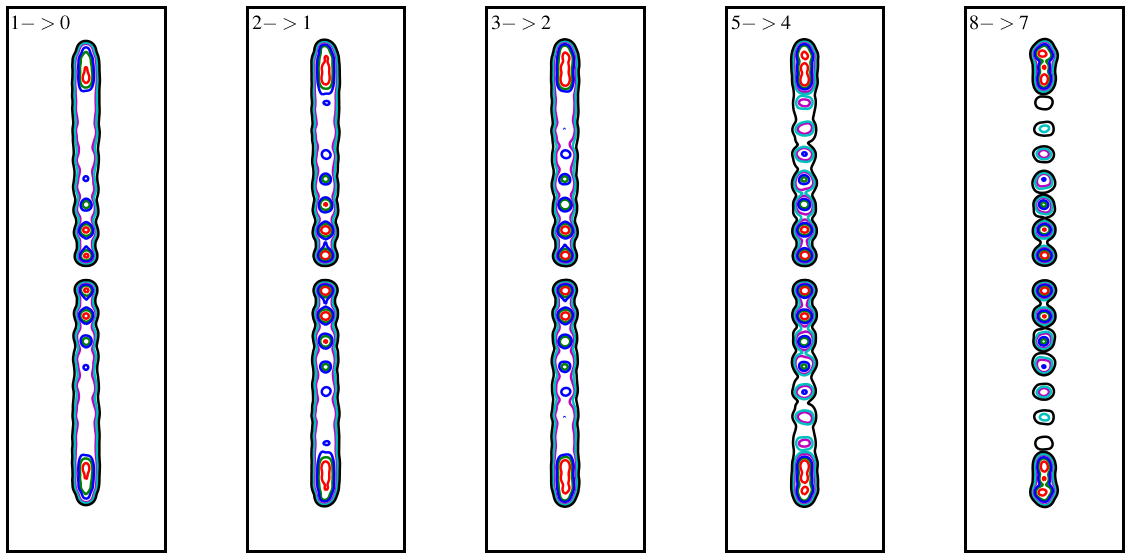
\includegraphics[width=2.\columnwidth]{\figpath/imshkvhcontomaps.png}
 \caption{Symmetrical contour maps of multi-line integrated SiO
   emission convolved with a 2\arcsec beam obtained using parameters of the reference run. The contour colors represent different intenties in Kelvins, i.e,
   20.0({\it red}), 10.0({\it green}), 5.0({\it blue}), 1.0({\it
     magenta}), 0.5({\it cyan}), 0.1({\it black}).} 
\label{fig:ltconts}
\end{figure*}

\cite{Nisini:2007p13128} have shown that the current
plane-parallel shock models fit reasonably well the physical
conditions traced by the SiO emission i.e., temperature $\lesssim$
1000\,K and H$_{2}$ number density $\sim$ 10$^{5}$-10$^{6}$
cm$^{-3}$, assuming optically thin emission. 
They can also fit the observed fractional SiO abundance of
$\sim$ 10$^{-7}$ in these outflows. However, they fail to predict all
the line profiles and in particular their similarities for low and
high excitation lines. Line emission for SiO from our model also traces similar
physical environment. Fig.~\ref{fig:Hmolform} shows that regions close
to the internal knot have temperatures up to 1000\,K and molecular
hydrogen density of the order of 10$^{6}$ cm$^{-3}$ (also see
fig.~\ref{grid}). These are the regions where the bulk of the SiO
emission is present, with fractional abundances between 10$^{-6}$ to 10$^{-8}$.
The line profiles shapes obtained from our study fit reasonable well with that observed by
\cite{Nisini:2007p13128}, especially for the bullets seen in
L1448. Interestingly, in our models, the line profiles are equally broadened for low as well
as high excitation lines. The top panel of fig.~\ref{fig:lineratio} shows spectra for three line
transitions for the reference run but with an angle of inclination
$\phi$ = 60$^{\circ}$ and convolved with a single dish beam of
15\arcsec to simulate observed integrated
intensities of L1448 bullets observed with large beams from JCMT and
IRAM. Intensities predicted from our model (see table~\ref{tab:result2}) lie within a factor of two
from the observed values (Table 2 of \citealt{Nisini:2007p13128}).
%


The variation of integrated single dish emission with upper transition
levels J$_{\rm up}$ for different abundance profiles is shown in the
right panel of fig.~\ref{fig:lineratio}. It is clear that the emission
obtained using a top hat profile is brighter than the one obtained
with a Gaussian SiO profile. However, curves obtained from
both these profiles show a very similar shape of a distinct rise followed by a fall in
integrated emission for higher transitions with a peak in
emission for J$_{\rm up}$ = 3. These curves helps to to predict the
hydrogen number density and temperature in outflows. Physical
conditions in outflows can also be studied by estimation of line ratios.
Values $\approx$ 1 for line ratios SiO(8-7)/(5-4) and SiO(5-4)/(2-1) have been
found in HH212 \citep{Cabrit:2007p13804,
  Lee:2008p13697} and also for molecular outflows from massive
young stellar object IRAS 17233-3606 (\citealt{Leurini:2013p13165}).
The local velocity gradient (LVG) slab modeling with optically thin approximation were unable to produce
these line ratios. 
In the present non-LTE radiative transfer modeling, no assumption of optical
depths or photon escape probability are prescribed and line ratios are
self consistently calculated and are shown in the bottom left panel of
fig.~\ref{fig:lineratio}. Their values lie very close to unity as
indicated from observations. 
%Further, we have estimated the optical
%depth in regions emitting SiO and find them to be optically thick with
%an optical depth $\tau \sim 10$. Thus, assuming optically thin SiO emission
%from molecular outflows especially from shocked dense knots would
%only provide upper limits. 
In summary, the shape, ratio and peak intensity of the spectra
obtained from our model fit very well to observed values implying
that SiO emission from our model is tracing the regions with right physical
conditions that are required to emit SiO in the gas phase via shocks. 

\begin{figure*}
 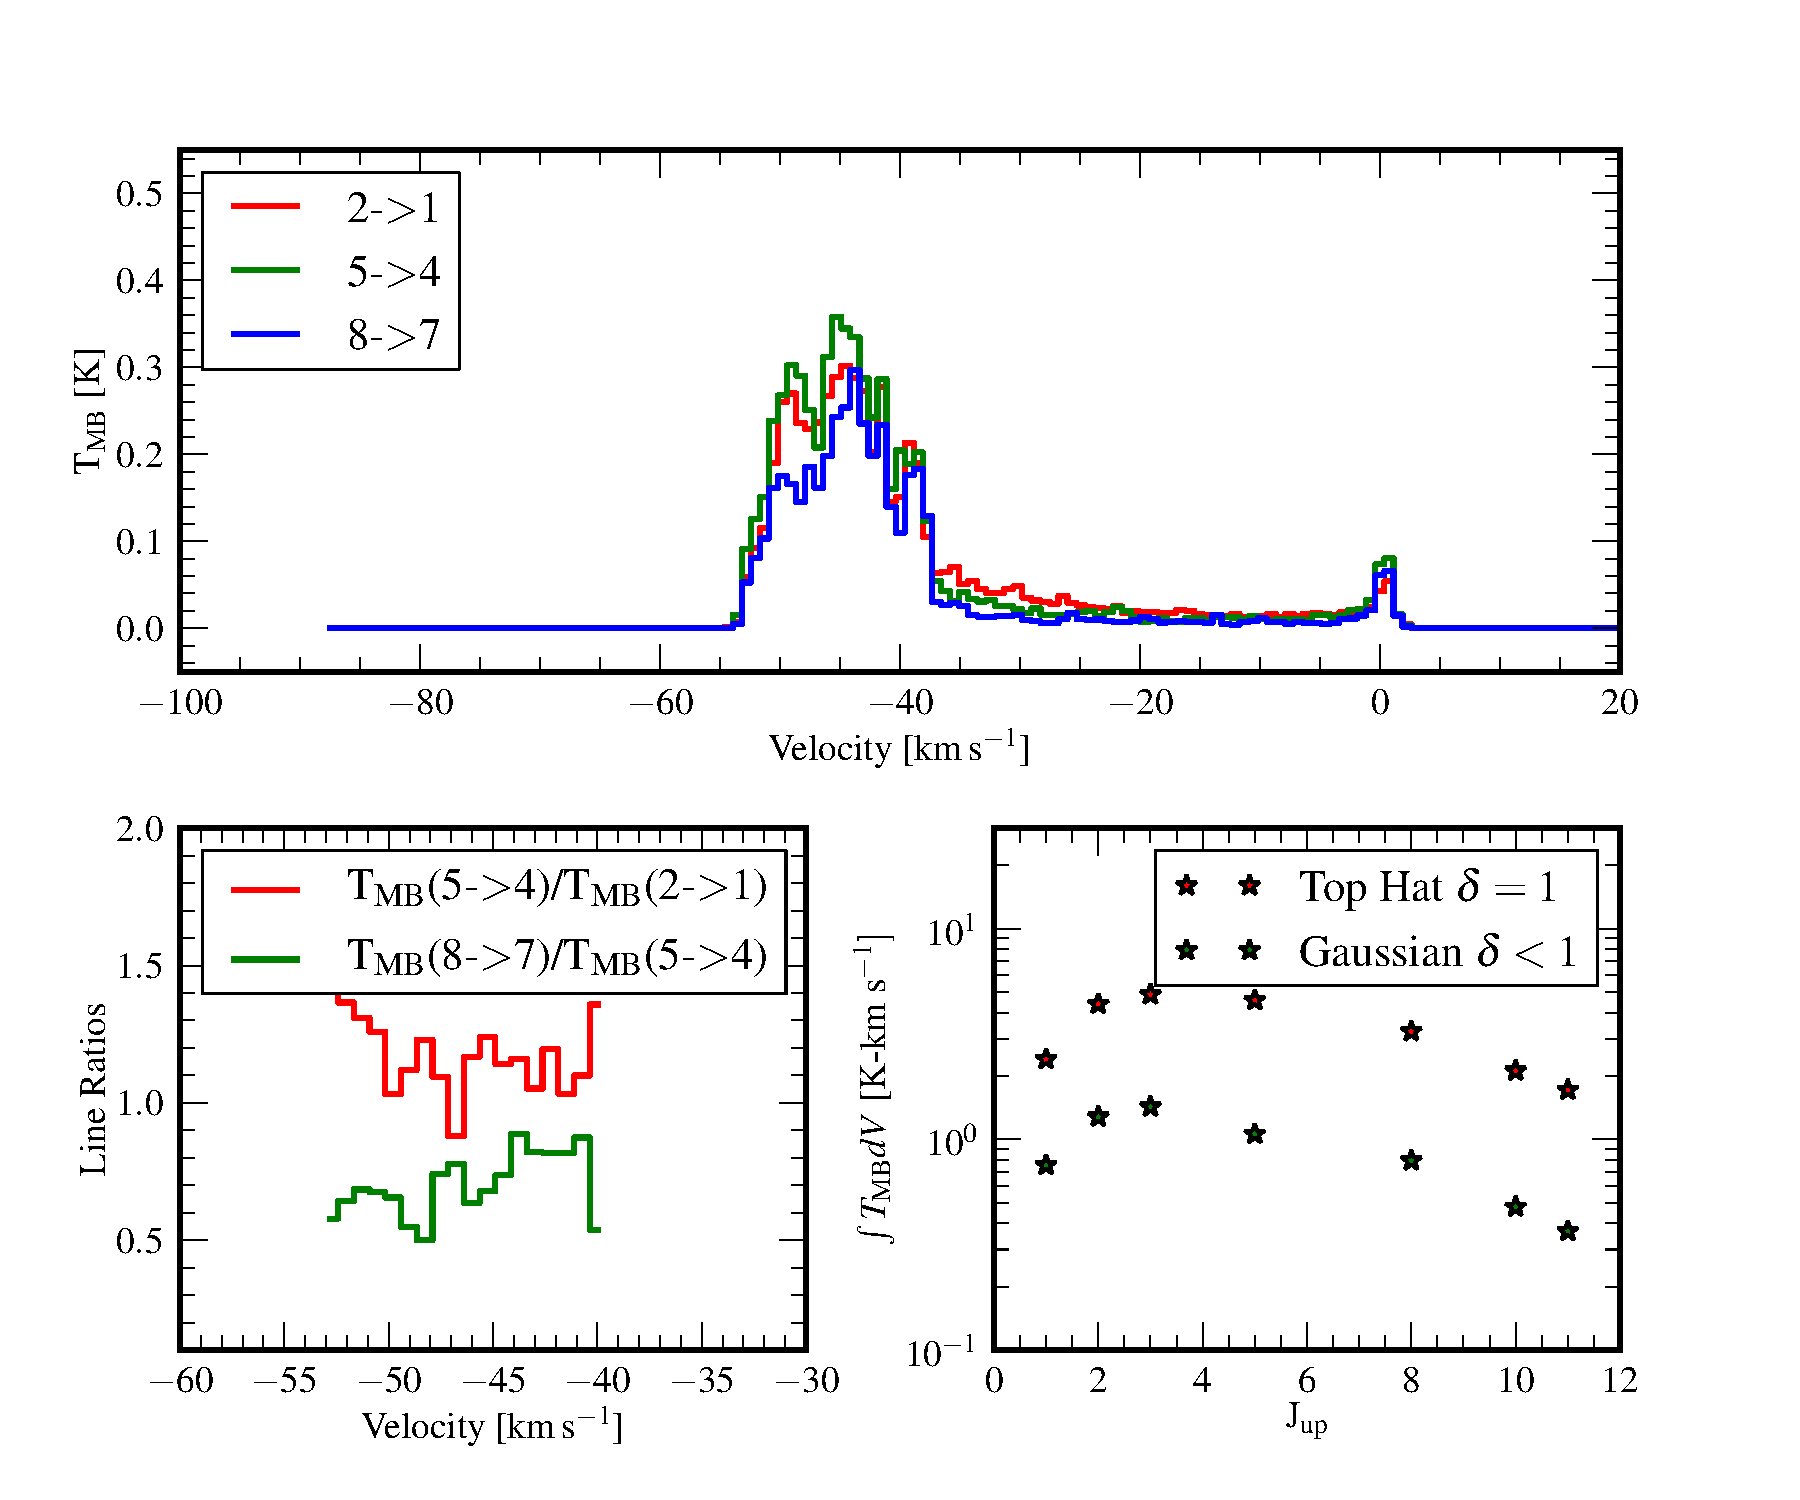
\includegraphics[width=2.\columnwidth]{\figpath/singledish_new.pdf}%{\figpath/LineRatio_THDeq1.png}
 \caption{{\em{Top}} Line profiles in SiO (2-1), (5-4) and (8-7) at one
   the inner knots for the reference molecular cooling run with a top
   hat abundance profile and $\delta = 1$. The profiles are
   obtained when the angle of inclination is 60$^{\circ}$ with respect
 to line of sight. {\em{Bottom left}} Line intensity ratios SiO(8-7)/(5-4)
and SiO(5-4)/(2-1), as a function of velocity. {\em{Bottom right}}
Variation of integrated intensity with upper line transition J$_{\rm
  up}$ for two abundance profiles.}
\label{fig:lineratio}
\end{figure*}


\subsection{Slow Component and Grain Chemistry}
%
We have presented a model that is able to explain the spectral characteristics
of the SiO EHV component seen
in several young outflows. The reference model
consistently solves for the H$_{2}$ chemistry in presence of
appropriate cooling. The steady state temperature, density and velocities obtained from dynamical
simulation is used as input in the non-LTE radiative transfer code to obtain SiO maps, spectra and PV
diagrams. One essential ingredient required for the radiative transfer modeling
is the SiO fractional abundance and its dependence on shock velocity. 
Though 1D models that study the formation of SiO in gas phase from grain-grain and grain-mantle
collisions exists, their focus is mainly on weaker shocks
\citep{Schilke:1997p14140, Caselli:1997p14853, Gusdorf:2008p13800, VanLoo:2013p16573}. 
The pulsating jet propagation model presented here have shock speeds
reaching up to 100 km\,s$^{-1}$. We have used few
simplified SiO abundance profiles as a function of shock
velocity. Though the shape of the profile is uncertain, the upper and
lower limits used are backed by observational evidences. Ideally, for a consistent
dependence of SiO abundance on shock velocity, one would have to also
solve for silicon and SiO chemistry in a manner similar to that of
H$_{2}$. However, such a numerically expensive model 
with complex chemistry is beyond the scope of this paper 
as this could imply to include dust grains and sputtering 
as well as grain-grain collisions (i.e. an MHD multi-fluid approach).  
%

The model presented in this paper targets the very early phases of molecular
outflows i.e., dynamical time scales of 1000 years.
As discussed in sections above, the unique combination of pulsating
jet with chemistry and cooling followed by non-LTE radiative transfer
calculations has shown success in fitting the line shapes, integrated intensity and line ratios of SiO
transitions arising from EHV gas. However, the synthetic spectra show
no signatures of slow SiO component that accompanies EHV emission seen
in many outflows \citep[e.g.,][]{Lefloch:1998p13983,
  Codella:1999p12584}. 
The physical mechanism for the origin of the slow SiO component is still a matter
of debate. \cite{Codella:1999p12584} suggest that it arises due to the slowing down of
shocked gas as they age. The time scale estimated for the shocked gas
to slow down is of the same order of magnitude as the SiO destruction
time scale i.e., 10$^{4}$ years (\citealt{Codella:1999p12584}). In this
case, we do not expect to see the slow velocity SiO component, as our
models stop at $\sim$ 1000 yr. However, we do see initial 
hints of slowing down of more evolved gas in terms of the velocity
shift of about 7-10 km\,s$^{-1}$ in peak emission between that
coming from the freshly formed internal knots close to the base of the
flow and that from the more evolved gas near the
bow shock. To ascertain this fact in more details, one would
need to track the bow shock for 10$^{4}$ years
using a larger simulation box and possibly with adaptive gridding 
which will be considered for future simulations. Such a long term
evolution will also help to provide a numerical model for the formation of HH objects
which are believed to be slowed down and more evolved forms of our
young molecular bullets, as suggested by \cite{Norman:1979p14858} and
  \cite{Hartigan:1987p11178}.
%

An alternative hypothesis for the origin of the low velocity SiO
component is that it could be formed by interaction of wider slow
shocks with the ambient medium. Generally it is assumed that the silicon material comes from dust
grain cores and that it is necessary to sputter or vaporise such cores
to obtain some SiO in gas phase. However, some silicon material may be
mixed with the ices on the dust grain surfaces (see discussion in \citealt{Schilke:1997p14140}) . In such a scenario, 
shocks with speeds below 20 km s$^{-1}$ might inject a significant
amount of silicon into the gas phase from the mantles, without 
completely destroying the grains. \cite{JimenezSerra:2010p15530} also found parsec-scale emission of SiO
toward an infrared dark cloud suggesting that large scale shocks (may
be triggered by cloud-cloud collisions \citealt{Henshaw:2013p15540}) may
be responsible.
Testing such scenarios is beyond
the scope of the present model. One would not only need proper
treatment of dust physics but also a two fluid model to study the impact
of slow shocks in two dimensions. These models are indeed very
important to study wide and slow emission from molecules like CO 
as seen in some young outflows like L1157 (\citealt{GomezRuiz:2013p14549})
and H$_{2}$O as seen from recent results of the Herschel-WISH survey
(\citealt{Tafalla:2013p12586}).

 
\section{Conclusion}
\label{sec:conclusion}
We have performed MHD simulations
of episodic radiative jet propagating 
with a typical speed of 100 km s$^{-1}$ into a cold, non-magnetized ambient
molecular medium with a density gradient. The jet dynamical quantities are evolved in conjunction
with different optically thin, non-equilibrium cooling prescriptions of varying complexities. 
The most complex is that of molecular cooling along with
H$_2$ chemistry. This prescription allows us to track the formation
and destruction of HI, HII and H$_2$ along with the flow dynamics. 
The final state of the jet obtained for each cooling model is then
used as input into a non-LTE radiative transfer code to
obtain SiO emission maps, spectra and PV digrams. The main results
obtained from our study are as follows :
\begin{itemize}
\item Different cooling prescriptions used for our model
  significantly influence thickness of the jet. An
  efficient mode of cooling does reduce the size of the cocoon and results
  in a more narrow jet. In addition, the bow shock structure
  differs with various cooling modes. Also, with realistic cooling
  functions one sees development of
  thermal instability at the jet head which also shows a significant emission in SiO
  along with young internal knots that are formed close to the base of
  the jet.
\item Emission maps obtained from our reference run with molecular
  cooling show a distinctive collimated outflow structure. The
  physical regions responsible of SiO emission in such early outflows
  typically have molecular hydrogen densities n$\sim$ 10$^{6}$
  cm$^{-3}$ and temperatures $>$ 500\,K which is consistent with
  properties deduced from LVG modeling of observational data of
  young outflows like L1448-mm.
\item Our multi-line study of SiO clearly shows how different
  line transitions are sensitive to different regions in the jets. For
  example, the SiO J = 1-$>$ 0 transition is mostly excited due to
  the interaction of the jet with the ambient medium, while SiO J = 8-$>$ 7 trace the inner most jet regions as
  they are excited only in the internal knots. This finding very well
  supports the multi-line observational surveys done for young
  molecular outflows, particularly, HH 211.
\item Single-dish synthetic spectra obtained from our model typically
  have intensity of 0.3\,K and peak around 50\,km\,s$^{-1}$ and have a
  typical line width of 20\,km\,s$^{-1}$. Such modeled spectra are in
  excellent agreement with characteristic features of EHV emission of
  SiO seen in young molecular outflows . In addition, the line ratios 
  T(8-7)/T(5-4) and T(5-4)/T(2-1), predicted from our models have values close to
  unity consistent with observations. Further,
  indications of the formation of the slow component due to the
  slowing down of the
  older knots is clearly seen as a shift of centroid velocities by
  7-10\,km\,s$^{-1}$ in the first 10$^{3}$ years of evolution.
\item The predicted PV diagrams from our models show a distinctive
  knot like features that are generally observed in outflows like IRAS
  04166+2706.
\item Emission from internal knots do depend on the chosen profile of
  the abundance. On one extreme where all the internal knots emit SiO  
  with a step profile with $\delta =$ 1 and a top-hat profile with
  $\delta < 1$, whereas, no emission in
  seen in knots when a gaussian profile with $\delta$ = 1 is used. For
  the remaining cases, we observe that emission mainly
  comes from knots close to the base of the flow and the condensation
  formed at the bow shock due to thermal instability.
\item Predicted ALMA maps also show characteristic features that are
  consistent with young molecular outflows with EHV emission. 
\end{itemize}

In summary, this work for the first time provides a model
that explains the origin of EHV emission seen in SiO from 
the inner regions of young molecular outflows. The unique combination
of axisymmetric jet propagation model with molecular cooling and
non-LTE radiative transfer calculations can successfully reproduce most
of the observed properties of SiO emission from young molecular
outflows. This model provides an excellent
template to compare current ALMA observations and can also predict
signatures of thermal instabilities which can be tested with upcoming
ALMA observations. In future, we would like to extend our
model to full three dimensions with adaptive mesh refinement
and evolve the jet for longer time scales to explore slow velocity 
component, precession and slew of other instabilities. Additionally, we would also like to have
a better handle on SiO abundance not only from observations but also
by including dust micro-physics in our model. 



%\section*{Acknowledgments}
%BV would like to thank everyone.

\appendix

\section{Treatment of Adiabatic Index $\gamma$}
\label{sec:treatgamma}
In dealing with a gas chemistry network which can have both monatomic and diatomic
species, one is immediately presented with the issue of how to treat the adiabatic
index, $\gamma$, of the gas, which directly influences the equation of
state, eq.~\ref{EOS}, and thus the behaviour of the gas.
In standard hydrodynamical codes the gas is generally
assumed to be a monatomic ideal gas, with $\gamma$ = 5/3. 
A diatomic gas, such as H$_{2}$, on the other hand, has a value of $\gamma$
= 1.4 at low temperatures, decreasing to below 1.3
at higher temperatures as the vibrational modes of the hydrogen molecule become
excited. Thus, the value of $\gamma$ for a gas containing a mixture of atomic and
molecular hydrogen requires a temperature-dependent calculation of the $\gamma$
value for H$_2$ and a weighting of the values for the atomic and molecular components
according to their abundance. \cite{Yoshida:2006p13376} have suggested
a prescription of an effective $\gamma$ which takes into account the
corresponding weights of each chemical species and is given by,
\begin{equation}
\frac{1}{\gamma_{\rm eff} - 1} = \frac{1}{\mu}\left[\sum_{i}\frac{X_{i}}{A_{i}}\frac{1}{(\gamma_{i} - 1)}\right]^{-1},
\label{eq:gammaeff}
\end{equation}
where, i is the index for each specie and $\mu$ is the mean molecular
weight. The mass fraction is added in the above equation following the
correction suggested in \cite{OSullivan:2009p10078}.
Additionally, the temperature dependence for example in case of
H$_{2}$ molecule can be obtained using \cite{landau:1980},
\begin{equation}
\frac{1}{\gamma_{H_{2}} - 1} = \frac{1}{2}\left[ 5 +
  2x^{2}\frac{e^{x}}{(e^{x} - 1)^{2}}\right],
\label{eq:gammaH2}
\end{equation}
where the last term with  x = 6100 $K$/T accounts for the vibrational
degree of freedom, with T being the gas temperature.
%

However, for such an implementation in large scale simulations one must first
consider its cost, effectiveness, and even correctness. Although such
a method would indeed yield a more correct $\gamma$ value for the gas
mixture in conditions where the rotational and vibrational modes have
had enough time to reach the level of excitation corresponding to
the temperature of the gas, in cases where the gas has just been
shocked, the method would produce an incorrect $\gamma$ value. 
This is because the gas that passes through shock gets rapidly heated, 
but this energy goes predominantly into the translational degrees of
freedom of the gas. It is only with time that energy goes into the rotational and
vibrational degrees of freedom of the gas through collisions. 
\cite{Flower:2003p11236} maintains that therefore the adiabatic index of
the post-shock gas has close to the ideal monatomic value of 5/3, 
and that in order to calculate correctly its evolution as the gas 
adjusts one would have to model the rotational and vibrational 
levels of the hydrogen molecules in a time-dependent manner.
%

For large-scale simulations present here it is more practical to use
the the standard value of 5/3 which is correct for the post-shock 
and predominantly atomic parts of the flow but incorrect for the
equilibrated parts of the flow with a significant fraction of molecular matter.
Since in this case, as the shock regions and their effect on the molecular hydrogen content of 
the ambient gas are of primary importance here, we opt for the more
relevant, and also simpler, policy of keeping the normal $\gamma$
value of 5/3 for our simulations. 

\section{Working surfaces and shocks}
\label{sec:worksurface}
In this section we describe the mathematical derivation of estimating
the speed of the working surface of the internal knot and shock speeds
associated with it. We will follow the derivation as given in
\citep{Raga:1990p16416,Raga:1992p16392}. Fig.~\ref{fig:interknot} shows a cartoon
representation of a single internal knot formed in the jet. 
The density and velocity upstream of the internal shock are
$\rho_{1}$ and $u_{1}$, while, the downstream values are $\rho_{2}$
and $u_{2}$ respectively. Note the velocities u$_1$ and u$_2$ are measured
in a stationary frame of reference of the star. The velocity of the working surface is
denoted by $v$, can be derived from the ram pressure balance between the upstream and
downstream flow,
\begin{equation}
\rho_1 (u_1 - v)^{2} = \rho_2 (v - u_2)^{2}.
\label{eq:ramPbal}
\end{equation}
This gives us the expression for $v$ as, 
\begin{equation}
v = \frac{u_1 + \zeta u_2}{1 + \zeta},
\label{eq:velws}
\end{equation} 
where, $$\zeta = \sqrt{\frac{\rho_{2}}{\rho_1}}$$.

\begin{figure}
\includegraphics[width=1\columnwidth]{\figpath/Internalknot.pdf}
\caption{Schematic diagram showing the structure of the internal
  working surface. The faster upstream material with velocity u$_1$
  catches the slower downstream material with velocity u$_2$ forming a
two shock structure (u$_2 >$ v $>$ u$_1$). The in-between gas is squeezed out sideways
forming the cocoon.}
\label{fig:interknot}
\end{figure}

The parameter $\zeta$ is obtained in principle from the two
dimensional snapshot of the jet density. In case of bow shock, the
downstream medium is the stationary ambient medium (u$_2$ = 0), thus,
eq.~\ref{eq:velws} will reduce to eq~\ref{eq:shockjetvel}.
However for the internal knots, the variation of density and
velocity for the reference run is shown in fig.~\ref{fig:1dvelrho}.
As can be clearly seen, the value of $\zeta \approx$ 1 for most of the
internal knots seen in our simulations. Thus, the velocity of the
working surface simplifies to, 
\begin{equation}
v = \frac{u_1 + u_2}{2}.
\label{eq:velwssimple}
\end{equation}

Additionally, the shock velocity (i.e, the velocity of the pre-shock
flow with respect to the velocity of the working surface) of the
upstream and downstream facing shocks have the same velocity given by \cite{Raga:1990p16416},
\begin{equation}
w = \frac{u_2 - u_1}{2} = 0.5\Delta u.
\label{eq:shkvelws}
\end{equation}

\begin{figure}
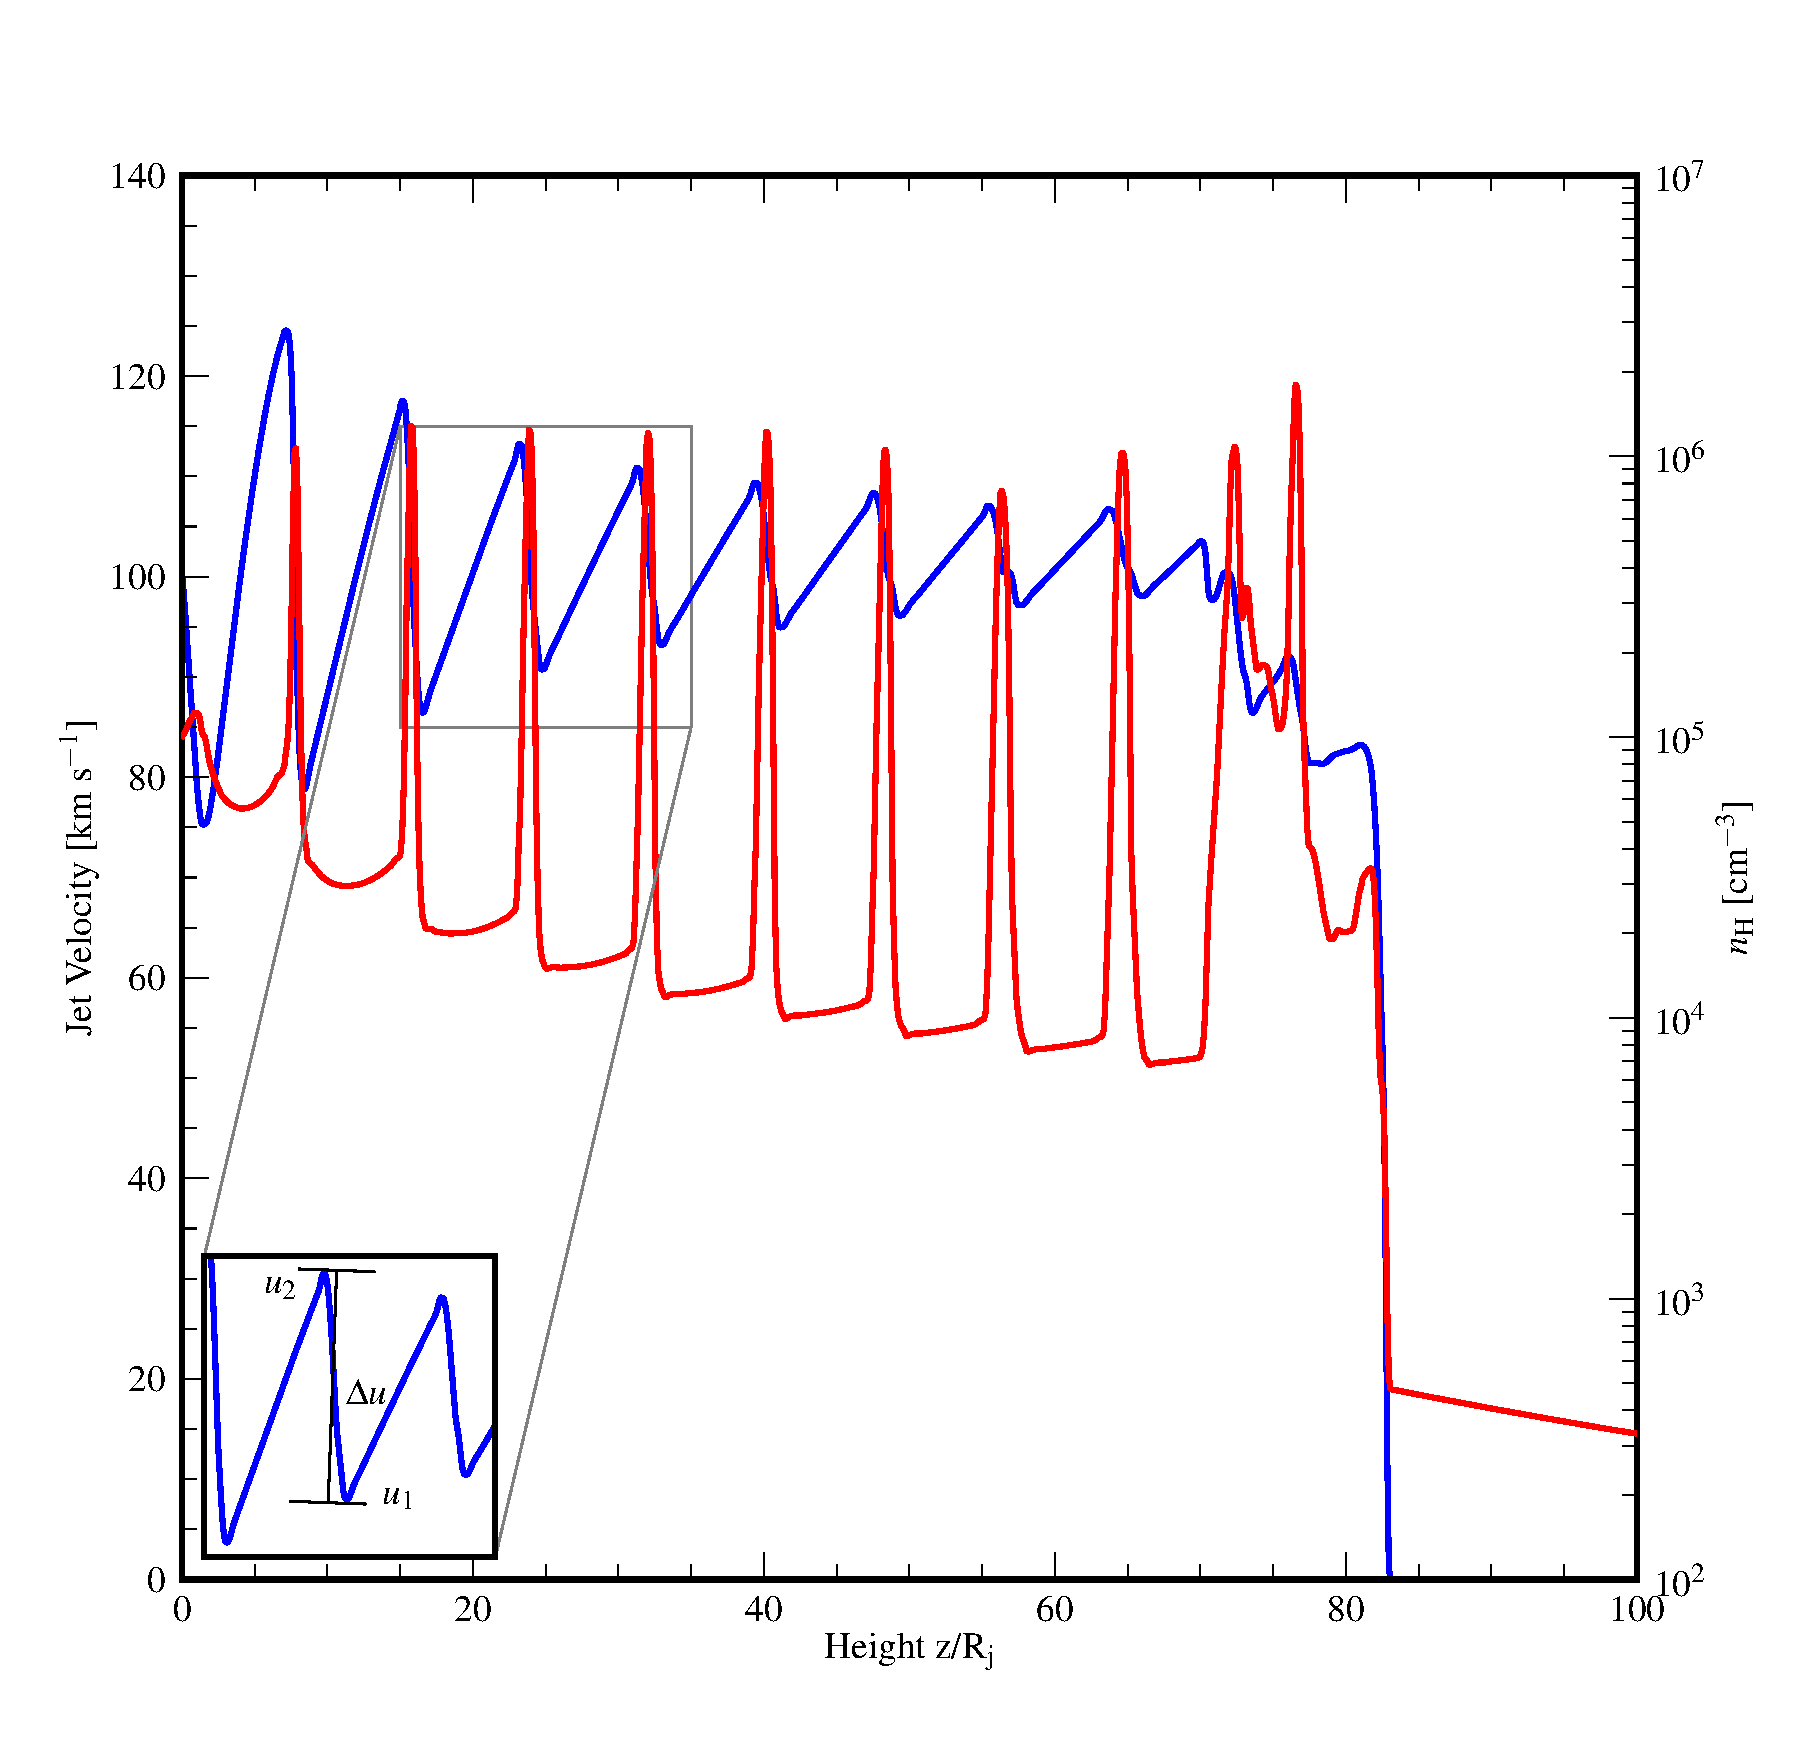
\includegraphics[width=1\columnwidth]{\figpath/jet_rhovel.pdf}
\caption{Variation of jet velocity (blue) and density (red) as a
  function of height close to the axis of the flow. The inset on the
  bottom left of the figure shows a zoomed variation of velocity and
  clearly marks the peak to peak difference between the upstream and
  downstream components.}
\label{fig:1dvelrho}
\end{figure}


The difference in the pre- and post-discontinuity velocities, $\Delta
u$ is marked clearly in the fig.~\ref{fig:1dvelrho}. Typically, the
difference in velocity values for our reference runs lie around 15-40 km s$^{-1}$. Thus, the
shock velocity $w$ lies around 10-20 km s$^{-1}$. Similar values are
also obtained for jets like HH 34 by \cite{Raga:1992p16392}.

The variation of SiO abundance used for the present model is rather
obtained from empirical values. In case of L1448, \cite{MartinPintado:1992p14309}
have shown that for extreme velocities (obtained from shift in the
spectra) of -40 to -50 km\,s$^{-1}$, the SiO abundance could be as
large as $6\times10^{-7}$, while, it slightly increases to
$2\times10^{-6}$ for the velocity range of -60 to -50
km\,s$^{-1}$. For the same source, typical {\em{shock}} (or working
surface) velocities of the {\em{molecular bullets}} are estimated to
lie around 80-175 km\,s$^{-1}$ \cite{Dutrey:1997p11185}.
\\
{\color{red}
WE HAVE TWO OPTIONS:\\ 
1. Since the there is a empirical evidence with bulk gas motion. We
can use just the jet velocity obtained from simulations.\\
OR\\
2. We can try to connect the working surface velocities from
\cite{Dutrey:1997p11185} to abundance obtained by
\cite{MartinPintado:1992p14309} and there by use the velocity of the
working surface as an independent variable on the X axis of the
abundance plot.
}





   
 

\newpage
\bibliographystyle{mn2e}
\bibliography{/Users/bhargavvaidya/MyProject/work/Leeds_Uni/SiOJets_New/PAPER/bibfile}
\label{lastpage}
\end{document}
